% This is samplepaper.tex, a sample chapter demonstrating the
% LLNCS macro package for Springer Computer Science proceedings;
% Version 2.20 of 2017/10/04
%
\documentclass[runningheads]{llncs}
%
\usepackage{graphicx}
% Used for displaying a sample figure. If possible, figure files should
% be included in EPS format.
%
% If you use the hyperref package, please uncomment the following line
% to display URLs in blue roman font according to Springer's eBook style:
% \renewcommand\UrlFont{\color{blue}\rmfamily}

\usepackage{enumerate}
\usepackage{marginnote}
\usepackage[linesnumbered,commentsnumbered,boxed]{algorithm2e}
\usepackage{amsmath}
\usepackage{threeparttable}
\usepackage[margin=0pt,skip=1pt]{subcaption}

\newcommand{\acumm}{T-Matrices} % T is for Total!
\newcommand{\ctr}{XCTR}
\newcommand{\ttctr}{TTCTR}
\newcommand{\ctrq}{XCTRc}
\newcommand{\ttctrq}{TTCTRc}

\begin{document}
%
\title{Next Trippy Structures\thanks{Supported by organization x.}}
%
%\titlerunning{Abbreviated paper title}
% If the paper title is too long for the running head, you can set
% an abbreviated paper title here
%
\author{First Author\inst{1}\orcidID{0000-1111-2222-3333} \and
Second Author\inst{2,3}\orcidID{1111-2222-3333-4444} \and
Third Author\inst{3}\orcidID{2222--3333-4444-5555}}
%
\authorrunning{F. Author et al.}
% First names are abbreviated in the running head.
% If there are more than two authors, 'et al.' is used.
%
\institute{Princeton University, Princeton NJ 08544, USA \and
Springer Heidelberg, Tiergartenstr. 17, 69121 Heidelberg, Germany
\email{lncs@springer.com}\\
\url{http://www.springer.com/gp/computer-science/lncs} \and
ABC Institute, Rupert-Karls-University Heidelberg, Heidelberg, Germany\\
\email{\{abc,lncs\}@uni-heidelberg.de}}
%
\maketitle              % typeset the header of the contribution
%
\begin{abstract}
The abstract should briefly summarize the contents of the paper in
15--250 words.

\keywords{First keyword  \and Second keyword \and Another keyword.}
\end{abstract}
%
%
%
\section{Introduction: sin hacer (queda para el final)}
We took the idea from our SPIRE paper and we made it great, using ZSTD compression and other tricks to improve the time complexity of the queries for the \ctr. Regarding \acumm, it was not possible to improve its speed (as it was already a few memory accesses per query), but we managed to compress it without increasing time complexity. We rock.

If possible, cite applications of our kind of analysis for transport/advertising companies, to show that what we are doing is useful. One example is \cite{tu2018spatial}. Another is \cite{zhang2017targeted}. And by the way, the guys in \cite{weng2018mining} do some analysis with data that has already boarding and alighting stops!

These guys \cite{wang2014aggregated} made it so boring that they are probably not worth citing, but I'm keeping them here for now because they separate fridays and types of days, even though we don't care much about that anymore. OR DO WE?

Aqui no estaria mal, ademas de motivar ;) completar con la estructura del paper, y de paso decir que es lo nuevo VS lo de SPIRE. (ej. Esta es una version extendida del X, donde hemos tratado de solucionar nuevas operaciones como x..., viendo que algunas de ellas se volvían ineficientes en el CTR original, decidimos realizar una nueva variante (\ctr), que permite responder más consultas eficientemente. Así, en la Seccion 2 T-R, en la seccon 3 - MODELO , en la seccion 4 mostramos nuestras propuestas y cómo utilizarlas para resolver consutlas... etc etc)



\section{Related works}
\subsection{Trajectory indexing}
Literature on spatial trajectory indexing can be categorized by the nature of the trajectories: they can be either constrained to a network or in free space (often called moving objects). While there are well-known queries for indexes that work on moving objects in free space \cite{DBLP:conf/vldb/PfoserJT00}, the network constrained trajectory indexes cover more diverse querying needs, as different networks involve different kinds of challenges (as in vehicular road network vs public transportation network), and also because the intended application may vary (analyzing trip-chaining patterns vs number of passengers within a time window). A comprehensive review on indexing methods can be found in \cite[Chapter 4]{DBLP:books/sp/PelekisT14}, to which we shall expand in the rest of this section to mention the most notable indexes and some new developments.

\subsubsection{Free trajectory indexing}
Several adaptations of the {\em R-Tree} \cite{DBLP:conf/sigmod/Guttman84} are widely used for the indexing of moving objects. The most common approach is to integrate the temporal dimension in the R-Tree itself, as found in the {\em STR-Tree} and the {\em TB-Tree} from \cite{DBLP:conf/vldb/PfoserJT00}.
Another common approach is to compliment the R-Tree with another similar structure, as has been done for the {\em MV3R-tree}~\cite{DBLP:conf/vldb/PapadiasT01},
where an Historical {\em R-Tree}~\cite{nascimento1998towards} to partition on the temporal dimension.

The observation that, even for free trajectories, temporal dimension is generally more selective than spatial dimensions was heavily exploited in the subsequent works, such as {\em SETI} from \cite{chakka2003indexing}, where the space is partitioned statically and the time is indexed with a one dimensional R-Tree.

Recently a framework based on Apache Spark was developed called {\em UlTraMan}~ \cite{ding2018ultraman}, that supports different kinds of partitioning schemes for large collections of trajectories to answer range, kNN or aggregation queries, allowing to repartition the dataset to maximize the query time efficiency for a given query type. Although UlTraMan has been tested over network constrained trajectories, it does not appear to be exploiting network information in any way, hence its inclusion in this category.

In the field of compact data structures, an index called {\em GraCT}~\cite{brisaboa2019gract} has been developed, based snapshots at regular time intervals using {\em k$^2$-Trees}~\cite{brisaboa2009k} and movement logs for individual trajectories to which grammar compression is applied with {\em RePair}~\cite{larsson2000off}. Because of this, GraCT is a self-indexed compact representation that supports spatio-temporal range and nearest-neighbor queries, as well as allowing for direct access to the trajectory information.

\subsubsection{Network constrained trajectory indexing}
There are also numerous approaches that use R-Tree based indexes for trajectories that are constrained to an underlying network, aiming to decrease the redundancy in the representation by separating the representation into levels. Examples of such indexes include the {\em FNR-Tree}~\cite{DBLP:conf/ssd/Frentzos03}, where the network elements are indexed with a 2D R-Tree and 1D R-Trees to index time intervals of moving objects along the edges of the network. Some of the limitations of the FNR-Tree are addressed in \cite{DBLP:journals/geoinformatica/AlmeidaG05}, where the authors propose the {\em MON-Tree}, where the moving objects are indexes in two dimensional R-Trees (the dimensions being edge position vs time). More recent alternatives, such as the {\em TMN-Tree}~\cite{chang2010tmn}, integrate {\em B$^+$-Trees}, which have proven to be more space and time efficient for indexing the temporal dimension. Alternatively, in \cite{rivera2018faster} a compact representation of time intervals is proposed using two bitvectors, that can be combined with these R-Tree based indexes to increase the efficiency for temporal filtering. Refer to \cite{john2017performance} for a quick comparison of these R-Tree based indexes.

As a competitive alternative to these R-Tree based indexes, {\em PARINET}~\cite{DBLP:journals/vldb/PopaZOBV11}, builds spatial partitions from the trajectories based on their distribution and network topology, and uses a B$^+$-Tree to index the trajectories in each partition by time intervals. Although candidate trajectories must be filtered in memory during queries, PARINET is highly efficient in practice as its partitioning strategy minimizes the number of disk accesses needed.
%The same ideas were used in {\em TRIFL}~\cite{that2015trifl}, where the cost model is adapted for flash storage.

Another relevant representation is described in \cite{DBLP:conf/gis/KroghPTT14}. Their proposed index, {\em NETTRA}, was designed to efficiently solve a specific kind of query called {\em Strict Path Queries (SPQ)}, built on a traditional RDBMS with $B^+$-Tree indexes. Another distinctive feature of NETTRA is its treatment of network constrained trajectories as textual information, which allows to apply string matching techniques such as fingerprinting functions to determine what trajectories have similar paths on their traversed edges. This close equivalence between trajectories and strings has been further exploited by Geodabs~\cite{chapuis2018geodabs}, where both the spatial distribution and sequence information are taken into account for finding trajectories by similarity with fingerprinting. These text-based approaches are sometimes tangled with works on the topic of semantic trajectories such as \cite{al2017semantictraj}.

%For vehicles we also have this \cite{cai2018vector} and \cite{lovell2018lossless}.

A recent compact data structure named {\em CiNCT} has been proposed in \cite{koide2018cinct}, where trajectories are encoded into a string, that is used to build an FM-index \cite{DBLP:conf/focs/FerraginaM00} with a Huffman-shaped Wavelet Tree \cite{ferragina2009compressed}. To further save space, the string is constructed with relative movement labels instead of absolute edges, with an auxiliary structure that represents a network graph built from the input trajectories themselves. While this structure excels at pattern-matching and path extraction in vehicular networks (such as the streets of a city), it cannot be applied to our problems in public transportation networks.

\subsection{Trajectory data mining}
Currently there are several known techniques that would allow to collect data regarding users' trips over a public transportation network. Numerous works exist where those trajectories are mined from the transactions of smart cards \cite{bhaskar2015passenger,wang2014aggregated}. This can be complemented with information derived from GPS devices, as shown in \cite{ma2014development}. Alternatively, reliable trajectories may be extracted relying on positioning obtained from cellular networks, as proven by \cite{liu2017exploring}.

In addition, the authors of \cite{tao2014exploring} have specifically tackled the challenge of reconstructing full trajectories, accounting for trip-chaining, by using data obtained from smart cards. Furthermore, in \cite{alsger2016validating} it is also proven that not only the alighting stops, but also the (last) destination stop of a trip can be estimated from boarding data gathered by a smart card, within a reasonable accuracy.

This summarized review proves that, although we were not able to access real data from a public transportation company for this work, such curated information about users' trips can indeed be obtained and used for our proposed representations.

\subsection{Underlying structures and algorithms}
\subsubsection{Summed Area Tables}
I mean maybe we should mention them :-)

\subsubsection{Bitvectors}
\label{sec:bit}
A great amount of works in Compressed Data Structures revolve around bitvectors, both compressed and uncompressed. For a bitvector $B[1,n]$ the following operations are expected to be supported:

\begin{itemize}
    \item $rank_1(B,i)$ returns the number of set bits in $B[1..i]$. Alternatively, $rank_0(B,i) = i - rank_1(B,i)$ and also $B[i] = rank_1(B,i-1) - rank_1(B,i)$.
    \item $select_1(B,i)$ returns the position in $1..n$ where the $i$th 1 occurs. Therefore, $rank_1(B,select_1(B,i)) = i$.
\end{itemize}

These operations can be supported in constant time with $o(n)$ extra bits \cite{Jac89,Mun96}, although several techniques exist for compressing bitvectors \cite{Raman:2002:SID:545381.545411,okanohara2007practical,Golynski2007}.

\subsubsection{Compressed Suffix Array (CSA)}
\label{sec:csa}
One common structure to count or locate all the occurrences of a pattern $P[1,m]$ in a string $S[1,n]$ of symbols from an alphabet $\Sigma$ is the Suffix Array (SA) \cite{MM93}. The SA lexicographically sorts all the suffixes $\{S[i..n] : 1 \leq i \leq n\}$ and builds an array $A[1,n]$ with their indices, holding that $S[A[i]..n] \prec S[A[i+1]..n]$. This allows to find out all the occurrences of a substring $P[1,m]$ in $O(m \log n)$ time with binary searches.

A simple enhancement to avoid storing the original string $S$ is to align $A$ with a bitvector $D[1,n]$ where $D[i]=1~\Leftrightarrow~S[A[i-1]] \prec S[A[i]]$. That is, $D$ marks with a 1 all the indexes $i$ of $A$ where the starting symbol of that suffix $S[A[i]]$ has a larger lexicographical value than the one from the previous suffix $S[A[i-1]]$. With $D$, keeping $S$ is not longer needed as $S[A[i]] = rank_1(D,i)$.
%, where $rank_1(D,i)$ returns the number of set bits in $D[1..i]$.

Sadakane's CSA \cite{Sad03} further reduces the space by replacing $A$ with a permutation $\Psi[1,n]$ \cite{GV00}, where given $A[i]=k$ and $A[j]=k+1$, $\Psi[i]=j$, while keeping the capability to count the occurrences of $P[1,m]$ in $O(m \log n)$ as the bitvector $D$ is still valid for the entries of $\Psi$. Although an uncompressed $\Psi$ would have the same space requirement as $A$, it is much more compressible as it is formed by $\sigma$ strictly increasing subsequences, being $\sigma$ the size of the alphabet $\Sigma$. Furthermore, it has been proved in \cite{NM07} that $\Psi$ can be split in $nH_k+\sigma^k$ (for any $k$) runs of consecutive values. It is therefore possible to compress $\Psi$ using $\delta$-encoding and run-length for the (frequent) runs of consecutive values. This property has allowed \cite{FBNCPR12}, among others, to achieve compression rates comparable to gzip for English text, while maintaining relatively fast random access by storing samples at regular intervals.

\subsubsection{Wavelet Matrix (WM)}
\label{sec:wm}
Based on the Wavelet Trees \cite{WT03}, the Wavelet Matrix \cite{CNO15} is a structure that is able to perform, given a sequence $S[1..n]$ over the vocabulary $\Sigma$, operations of $rank_a(S,i)$ and $select_a(S,i)$ $\forall a \in \Sigma$ in $O(log\sigma)$ time while using $n\lceil log_2\sigma\rceil~+~o(n)$ bits of space, begin $\sigma = |\Sigma|$.

The WM is built with $\lceil log_2\sigma\rceil$ levels, each level having a bitvector $B_i$ with rank and select capabilities, where $B_1$ contains the most significant bit of every symbol $a \in S$, $B_2$ contains the second most significant bit and so forth. To further explain how these bits are positioned, we must consider $a_i$ as the $i$th bit of $a$ in significance, and $B^{-1}_i[a_i]$ as the position of the bit $a_i$ from $a$ in the bitvector $B_i$. Then, 
\[
    B_i[j] = \left\{\begin{array}{lr}
        S[j]_1, & \text{iff } i=1\\
        a_i, & \text{iff } i>1 \wedge (a_{i-1}=0 \wedge j=rank_0(B_{i-1},B^{-1}_{i-1}(a_{i-1}))) \\
        & \vee~(a_{i-1}=1~\wedge~j=rank_0(B_{i-1},n)~+~rank_1(B_{i-1},B^{-1}_{i-1}(a_{i-1})))
        \end{array}\right.
\]

That is, $B_1$ contains all the bits $a_1 \forall a \in S$, in the same order as in S. After that, $B_2$ contains the $a_2$ bits from those $a$ such as $a_1 = 0$ first, followed by those with $a_1 = 1$. That way, all the position of each $a_i$ in $B_i$ depends first by the value of $a_{i-1}$ and later by their position in $B_{i-1}$. Refer to the structures \texttt{WML} and \texttt{WMJ} in Figure~\ref{fig:example_xctr} for examples of one and two-leveled WM. Additionally, there exists a conceptual \textit{leaf level}, that is formed by the final position of every $a$ after applying the recursion on the last level. Because the sorting of each level depends on the values of the previous most significant bits, in the leaf level all symbols are sorted by their reverse representation in bits.

This structure allows to answer the following operations in $O(\log\sigma)$ time:
\begin{itemize}
    \item $access(S,i)$ returns the value in any position in the original sequence $S$ by following through the levels of the WM using the $rank$ operation on bitvectors. If $B_1[i]$ is 0, then $B_2[rank_0(B_1,i)]$ must be accessed next. Otherwise, it is $B_2[rank_0(B_1,n) + rank_1(B_1,i)]$. This must be recursively applied until the leaf level is reached, and the traversed bits will compose the value of $S[i]$.
    \item $rank_a(S,i)$ is calculated with the same operations as in $access$, with the difference that in this case we know whether we need to use $rank_0$ or $rank_1$ on each bitvector as the value of the symbol $a$ is known. To calculate the number of occurrences of $a$ in $S[1..i]$ we must simply subtract the position reached in the leaf level to the position of the first occurrence of $a$ on that level, which can be either stored for each symbol in $O(\sigma\log n)$ bits or calculated by making an analogous traversal from the first position of $S$.
    \item $select_a(S,i)$ first $i$ must be added to the first position of $a$ in the leaf level, which as for $rank$, can be either stored or calculated. After obtaining this position $j$, the WM must be traversed in reverse order using $select$ on bitvectors until the first level is reached. When $a_i=0$ the traversal from the lower level position $B_{i+1}[j]$ must be as $select_0(B_i,j)$, while when $a_i=1$, it is done as $select_1(B_i,j-rank_0(B_{i},n))$.
    \item $range_{a,b}(S,i,j)$ returns the number of occurrences of the symbols between $a$ and $b$ in $S[i..j]$. This operation was first introduced in \cite{gagie2012new} for Wavelet Trees and later supported by the Wavelet Matrix \cite{CNO15}, and we make extensive use of it in this work. It is solved with two simultaneous traversals similar to $rank$ over $i$ and $j$, only that it is possible that at some levels it is required to calculate both $rank_0$ and $rank_1$. However, the worst case time complexity of $O(\log\sigma)$ is maintained, due to the fact that it is not necessary to reach the leaf level for all the symbols in $a..b$\footnote{As long as $a\neq b$. Otherwise, $rank_a(S,j)-rank_a(S,i)$ can be used.}.
\end{itemize}

While a compression method is proposed in \cite{CNO15} by using canonical Huffman encoding on the symbols, it could not be applied in our work because it severely reduces the efficiency of $range_{a,b}(S,i,j)$. Instead, we focused on compressing the bitvectors and using ad-hoc optimizations to reduce the average height of our WMs.

\section{Our model for compact trip representation}
In our previous structures introduced in \cite{brisaboa2018new}, we propose a work-in-progress model to represent the demand information for a public transportation network, as seen in the Figure~\ref{fig:er}.

\begin{figure}
%\centering
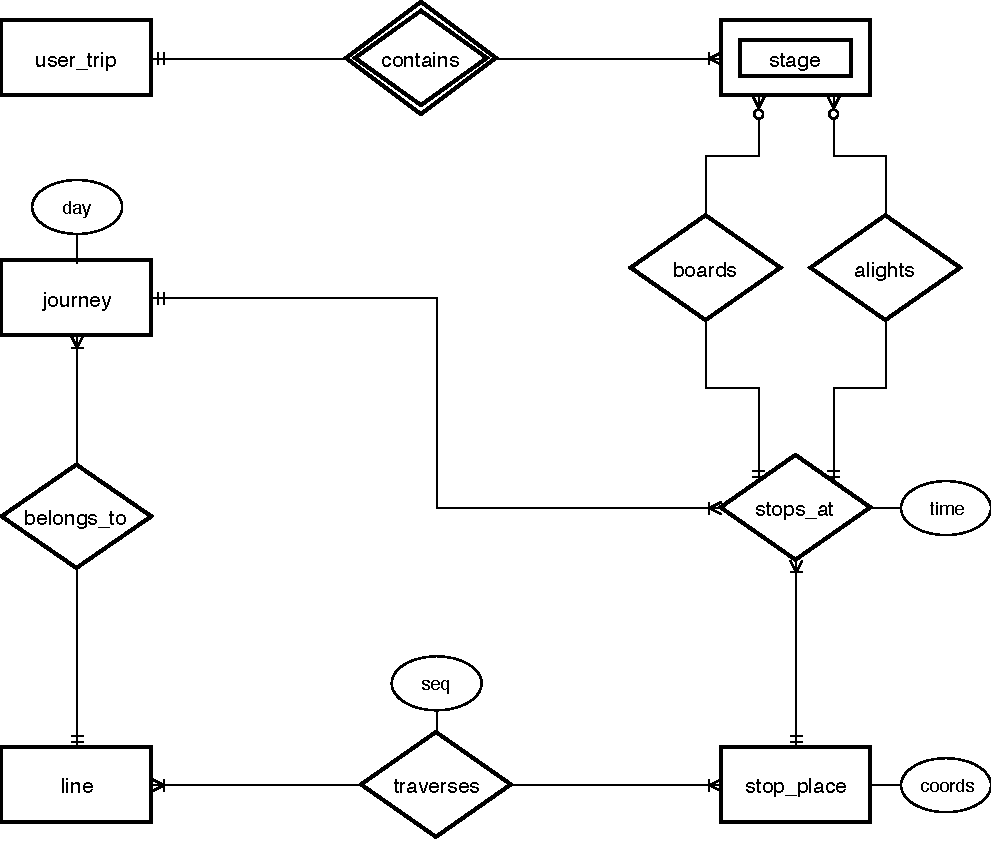
\includegraphics[width=\textwidth]{NetworkER.pdf}
\caption{An (updated) ER diagram representing the work-in-progress model for user trips in public transportation}
\label{fig:er}
\end{figure}

These are the main elements from our model:
\begin{itemize}
    \item A \textbf{stop\_place} is a physical stop with a location, on which several lines may make stops.
    \item A \textbf{line} is an ordered sequence of stop places that can be traveled by a transport vehicle, such as a bus or a train. It only considers one direction. For this reason, there is often a different and complementary line for the opposite direction, as shown in the Figure~\ref{fig:example_network}.
    \item A \textbf{journey} is a singular traversal of a transport vehicle over a line. It can be seen as a vehicle trip, instead of a user trip.
    \item A \textbf{stage} is formed by a boarding from a stop and alighting to another from the same single line and journey.
    \item An \textbf{user\_trip} is a concatenation of several stages, until the final destination (alighting stop of the last stage) is reached.
\end{itemize}

\begin{figure}
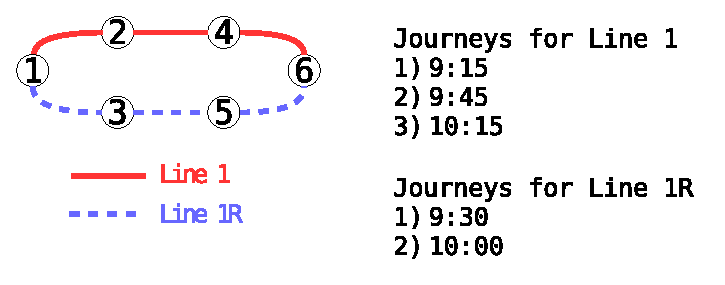
\includegraphics[width=\textwidth]{example_network.eps}
\caption{An example network for our model, with two lines and six stops}
\label{fig:example_network}
\end{figure}

This approach allows us to treat the information in a layered fashion: the bottom layer is a static network representation, formed by the line and stop\_place entities, the middle layer are the journeys made by vehicles that make stops at specific times, while the top layer are the trips made by the users over these vehicle journeys. In the Figure~\ref{fig:example_network} we show an example for the two bottom layers, where Line 1R is the reversed of Line 1. Our proposed implementation can be found in Section~\ref{sec:ps}.

Finally, it is possible to introduce a \textbf{user} identity, with an anonymized identifier to segregate trips by users. However, we do not consider such information useful for the kind of analysis that this work focuses on. If needed in the future, this additional entity could be trivially integrated in our representation.

\subsection{Relevant queries}
\label{sec:rq}
In the context of public transportation networks, we are interested in solving two kinds of queries:

\begin{enumerate}[A)]
    \item Aggregation of passengers, asking for the gross number of users that boarded or alighted within an area and a time window. Furthermore, it can be also interesting to obtain the average load of a bus or a train between any two stops from its line.
    \item Movement patterns, or queries that focus on the sequence of trip stages. Examples of such queries are the number of times a stop was used to switch lines or the number of trips that started on a stop with another specific stop as the final destination. 
\end{enumerate}

The following is a non-comprehensive list of query types that can be efficiently solved with the structures proposed in this work:
\marginpar{\tiny Nieves: Reorganizar seguindo a clasificación}
\begin{itemize}
    \item \texttt{board\_X$_{LT}$} Number of times that stop X is boarded, optionally restricting to a line L and a time range T.
    \item \texttt{alight\_X$_{LT}$} Number of times that stop X is alighted, optionally restricting to a line L and a time range T.
    \item \texttt{start\_X$_{LT}$} User trips starting at a stop X, optionally restricting to a line L and a time range T.
    \item \texttt{end\_X$_{LT}$} User trips ending at a stop X, optionally restricting to a line L and a time range T.
    \item \texttt{switch\_X$_{LT}$} Number of trips in which the stop X was used to switch lines, optionally restricting to a line L and a time range T.
    \item \texttt{from\_X$_{LT}$\_to\_Y$_{LT}$} User trips that originate at stop X to end at stop Y, both being optionally restricted to a line and time range.
    \item \texttt{board\_L$_T$}  Number of times that line L is boarded, optionally restricting to a time range T.
    \item \texttt{alight\_L$_T$} Number of times that line L is alighted, optionally restricting to a time range T.
    \item \texttt{start\_L$_T$} User trips starting at any stop from the line L, optionally restricting to a time range T.
    \item \texttt{end\_L$_T$} User trips ending at any stop from the line L, optionally restricting to a time range T.
    \item \texttt{board\_T} Number of times a user boards within a time range T.
    \item \texttt{alight\_T} Number of times a user alights within a time range T.
    \item \texttt{start\_T} User trips starting within a time range T.
    \item \texttt{end\_T} User trips ending within a time range T.
    \item \texttt{load\_X$_{LT}$} The average number of passengers traveling from the stop X to its next stop in the line L within the time range T. Can also be seen as the average load of a transport vehicle.

\end{itemize}

\section{Proposed Structures}
\label{sec:ps}
As of today, we are not aware of any indexing structure that would allow to efficiently represent trajectories that could also support all the kinds of queries described in Section~\ref{sec:rq}. For this reason, we propose two data structures, \acumm~and~\ttctr. The former is targeted for queries of type A, solving most aggregation queries in constant time, while the later can be used for queries of type B. Finally, we introduce a more versatile alternative to \ttctr~that we call \ctr.

\subsection{Common Structures}
\label{sec:cs}
Both \acumm~and \ttctr~need a network representation to be operated, along with information about the transport vehicle journeys. Therefore, the following structures represent a network with stops $s_i \in S = \{1,...|S|\}$, lines $l_i \in L = \{1,...|L|\}$ and journeys $j_i \in J^l = \{1,...|J^l|\}$. It is important to state that journeys are \textbf{not} identified by $j_i$, as the same $j_i$ can belong to several $J^l$ from different lines, so we speak about journey \textbf{codes} (jcodes) instead of journey identifiers.

\begin{itemize}
    \item $lineStop_i(j)$ is the $j$th stop of line $l_i$
    \item $stopLine_i(j)$ is the $j$th line that makes a stop at the stop $s_i$
    \item $avgTime_i(j)$ is the average time in seconds that it takes for a vehicle of line $l_i$ to reach its $j$th stop from the start of a journey
    \item $initialTime_i(k)$ is the starting time of the journey $j_k$ for line $l_i$
\end{itemize}

With the exception of $initialTime$, all these structures are small enough to be represented using plain fixed-length integer arrays. In the case of $initialTime$, its size naturally grows with the amount of trips that are indexed, thus there is a motivation to reduce its size, which can be easily achieved with any technique that works on posting lists or sequences of strictly increasing numbers. In our work we used a simplified Vbyte+ANS compression described in \cite{moffat2017ans} using the Zstd library\footnote{https://github.com/facebook/zstd}. In order to facilitate searches and random access, we introduced fixed-length samples on configurable intervals.

An example of these structures interacting together can be found at the Algorithm~\ref{alg:jcodes}, the the function \FuncSty{lower\_bound} is a binary search that returns the index of the first occurrence that is no lesser than the queried value, while \FuncSty{upper\_bound} returns the index of the last no greater occurrence.

\begin{algorithm}[H]
\SetKwData{l}{$l$}\SetKwData{lz}{l$_z$}\SetKwData{s}{s}\SetKwData{sz}{s$_z$}\SetKwData{ta}{t$_a$}\SetKwData{tz}{t$_z$}\SetKwData{pattern}{pattern}\SetKwData{left}{left}\SetKwData{right}{right}\SetKwData{csa}{CSA}\SetKwData{wmj}{WMJ}\SetKwData{leftzero}{left$_0$}\SetKwData{rightzero}{right$_0$}\SetKwData{i}{i}\SetKwData{z}{z}\SetKwData{ja}{j$_a$}\SetKwData{jz}{j$_z$}\SetKwData{n}{n}\SetKwData{ap}{a'}\SetKwData{zp}{z'}\SetKwData{offset}{offset}
 \SetKwFunction{GetBounds}{GetBounds}\SetKwFunction{GetJCodes}{GetJCodes}\SetKwFunction{GetCount}{GetCount}\SetKwFunction{GetPsi}{$\Psi$}\SetKwFunction{GetRangeSpecial}{GetRange$^*$}\SetKwFunction{bsearch}{binary\_search}\SetKwFunction{lbound}{lower\_bound}\SetKwFunction{ubound}{upper\_bound}
 \SetKwProg{Fn}{Function}{\string:}{}
 
 \Fn{\GetJCodes{\l,\s,\ta,\tz}}{
 \KwData{line \l, stop \s, times \ta,\tz}
 \KwResult{jcodes for \ta and \tz}
 \BlankLine
 \offset $\leftarrow$ $avgTime_{\l}(\bsearch{$lineStop_\l$, \s})$\;
 \Return{\lbound{$initialTime_\l$, \ta-\offset}, \ubound{$initialTime_\l$, \tz-\offset}}\;
 }
 
 \caption{Obtaining the codes of the journeys from the line \l that should arrive to the stop \s within the time range given by \ta and \tz}
 \label{alg:jcodes}
\end{algorithm}

\subsection{\acumm}
\label{sec:acumm}
As it has been stated previously in this paper, nowadays it could be relatively simple to gather massive information about user trips in every public transport; however, it is not necessary to store individually each trip. If there are two (or more) commuters sharing the same bus (train/tram/etc), they are also sharing the route, the stops (the time of each stop) and even the network. Therefore, a structure storing the aggregated data of the user trips would be a handy solution to solve (at least) queries of type A presented in section 3.

Thus, we propose the T-Matrix, an accumulated solution that involves two-dimensional matrices of integers enabling aggregated queries by row, column, or window/range. In the context of a public trasnportation network, it would by useful to solve flexible line-centered queries; that is, queries that support aggregation by any dimension. Therefore, it could be possible to aggregate either by time-interval (e.g. number of users got on at any stop of the line on 2019/01/02); by stop (e.g. number of commuters that got on a bus at stop S); or by stop and time-interval.

In a naïve representation, it would only be necessary a two-dimensional matrix having stops as rows and journeys as columns, so each cell would have an integer representing the number of passengers that got on the vehicle at a specific stop in a particular time (journey). The main issue with this approach is that for each query it would be necessary to sum integer by integer each cell of the solution; hence, if we are trying to compute how many people got on a bus in several consecutive stops during a time interval (several consecutive journeys) it would be necessary to sum all the cells within the matrix that match these journeys and stops.

On the other hand, T-Matrix is based on this naive proposal but instead of storing each cell as a simple integer it assigns an accumulated value to each slot, being the top left cell the smaller number and the bottom right position the cumulative value resulting from adding all the previous cells. Despite having larger numbers in almost every slot of the matrix, this approach allows to apply the dynamic programing formula that follows:

$\mathsf{countRange((x_1,y_1),(x_2,y_2))} \leftarrow {M(x_2,y_2)} - {M(x_2,y_1-1)} - {M(x_1-1,y_2)} + {M(x_1-1,y_1-1)}$.

The combination of this operations with our proposed accumulative matrix enables to compute the same two-dimensional (or one-dimensional) queries in constant time O(1), as it is only neccesary to access and sum four cells in all the matrix.

EXAMPLE

One simple way of dealing with the growth of numbers in our cumulative solution is just apply a kind of sampling with differences; in this way, a basic example could be keep the middle column m ← (n s + 1)/2 explicitly, and representing the values in the other columns m±k as the difference with respect to column m.



Taking this simple structure one step further we have built a cumulative matrix with several sampling columns, reducing significantly the size of the structure. Hence, this new cumulativematrix is divided in blocks having n-factor sampling columns, calculating n-factor as a percentage
of the total number of columns. During the queries real numbers in the matrix are obtained by adding each cell plus the nearest sampling column on the left.



In order to reach a lighter solution we combined the two last compression techniques building a cumulative matrix sampled by columns which have a centered sampled column in turn. Thus, a value in a cell of the matrix would be obtained adding its value to the value of the nearest sampling column on the left which would be calculted by summing this sampled value to the center column.



Due to comparison reasons it has been also built these sampled structures using sampling rows instead of sampling columns as it was explained, leading this to the the seven structures that have been used in the experiments of this work: the basic matrix (BASIC), the cumulative matrix (SUM), the cumulative matrix with a central sampling column as reference (DIFF), the cumulative matrix with several sampling columns that divide it in blocks (COL-BLOCK), the COL-BLOCK matrix with a second central sampling (COL-BLOCK-DIFF) and the row version of the last two, ROW-BLOCK AND ROW-BLOCK-DIFF respectively.


\subsection{\ttctr}
A user trip can be represented by the stops from the transportation system that were boarded by a user, so from now on we will consider a trip as a sequence of triplets $<s,l,j>$, where $s$, $l$ are, respectively, stop and line identifiers, while $j$ are the journey codes corresponding to the journeys that compose the trip. These triplets describe a trip in a consecutive fashion, on the same order as the stops were boarded. Additionally, as we are interested in knowing where the trips end, we also represent the last stop where the user has alighted, which line and journey will logically match the line and journey of the last boarding stop. Although it is generally hard to obtain information about the last destination stop of a trip, many transportation companies are investing effort in providing it, either by implementing systems to keep track of users as they leave their system or estimating it based on previous trips made by that user \cite{alsger2016validating}.

\ttctr~was introduced in \cite{brisaboa2018new}, where the spatial component (the pairs $(s,l)$ for the stops and lines of a trip) is represented with a \texttt{CSA} where each unique pair $(s,l)$ is encoded as an integer $id$ in the input sequence $T[1,n]$ that is used to build the \texttt{CSA}.

In this work, \ttctr~is built first by sorting all trips. If we consider that a trip is composed by $n$ of the $<s_i,l_i,j_i>,~1\leq i\leq n$ triplets previously described, where the first triplet corresponds to the first boarded stop and the last triplet corresponds to the last alighted stop (final destination), then the collection of trips is sorted by the key $s_1,s_n,l_1,j_1$. That is, trips are initially sorted by the first boarded stop identifier. If these are equal, they are then sorted by their last stop identifier, analogously followed by the line identifier and journey code of the first stop. Figure~\ref{fig:example_trips} displays an example of a correct sorting of trips.

\begin{figure}[hbt!]
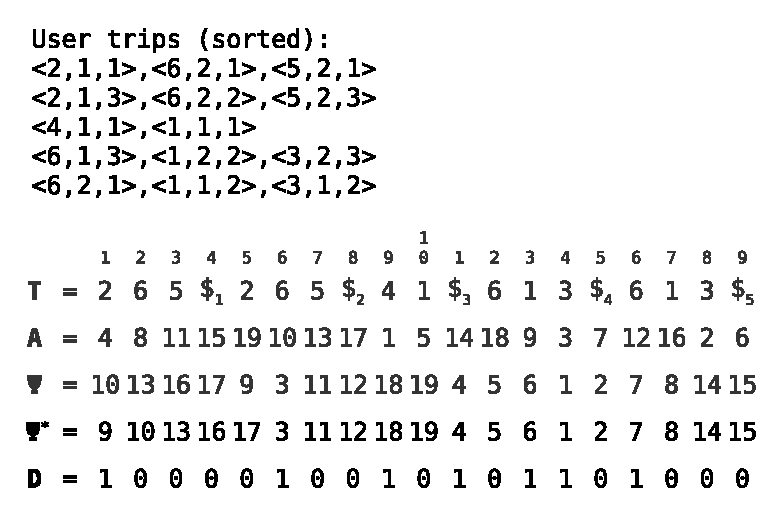
\includegraphics[width=0.4\textwidth]{example_trips.eps}
\caption{An example five trips sorted as required by \ttctr~and \ctr}
\label{fig:example_trips}
\end{figure}

We also need an injective function to encode the pairs $(s,l)$. Consider a vocabulary $V$ such that:
\begin{itemize}
	\item Entry $V[0]$ is reserved for the terminator symbol $\$$.
	\item Entries $\langle V[1],V[2], \dots V[|S|]\rangle]$ are associated to stops $s_1,s_2,\dots, s_{|S|}$ and are used to represent the final stops of the trips. That is, when a given stop $s_i$ ends a user trip, it is given $id \leftarrow s_i$.
	\item The following $|L|$$\times$$|S|$ entries are associated to the sequence composed of the pairs $(s,l) \in S\times L$, sorted first by the stop id $s$ and later by the line id $l$. That is, entry $V[|S|+1]$ is given to $(s_1,l_1)$; $V[|S|+2]$ to $(s_1,l_2)$; $V[|S|+3]$ to $(s_1,l_3)$; $\dots$; $V[|S|+|L|]$ to $(s_1,l_{|L|})$;  $V[|S|+|L|+1]$ to $(s_2, l_1)$, $V[|S|+|L|+2]$ to $(s_2, l_2)$, and so on. Therefore, it is easy to see that any $(s_i,l_j)$ is going to be associated to the entry $V[|S|+ |L|(i-1) + j]$.
\end{itemize}

While this arrangement would theoretically produce many entries in $V$ that are mapped to pairs $(s,l)$ that are unused in $T$, either because the stop is never traversed by that line or because we do not have the record of a user trip containing it, these entries can be skipped with a compact bitvector $B$ with rank and select capabilities, that marks with a one every used entry from $V$. This will enable us to operate with a much smaller vocabulary $V'$ with only the used entries from $V$, such that $V[i] = V'[rank_1(B,i)]$. Refer to the vocabulary shown Figure~\ref{fig:ttctr}(2) for an example where pairs $s:l$ are encoded to 43 unique identifiers in $V$. After that, $B$ marks which of the entries of $V$ actually appear in the original sequence. Finally $V'$ will contain only 12 entries, for each set bit from $B$. Note that neither $V$ nor $V'$ are explicitly represented in practice, as $rank$ and $select$ operations over $B$ are enough to map and unmap, respectively, vocabulary identifiers.

\begin{figure}
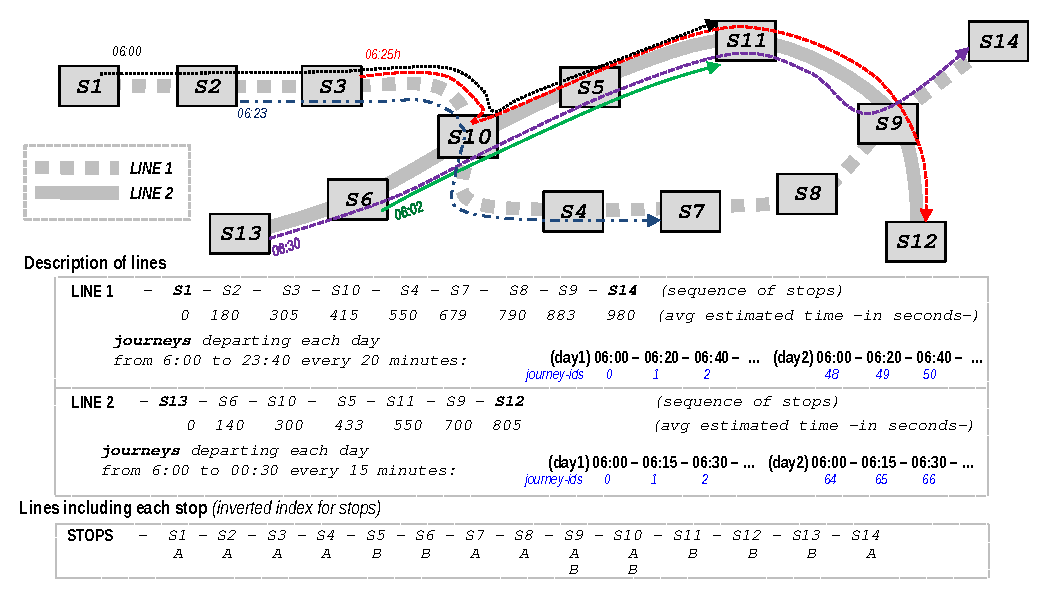
\includegraphics[width=\textwidth]{network.eps}
\caption{Network representation for the example of \ttctr~from Figure~\ref{fig:ttctr}}
\label{fig:example_trips_ttctr}
\end{figure}

\begin{figure}
	%\vspace{-0.2cm}
    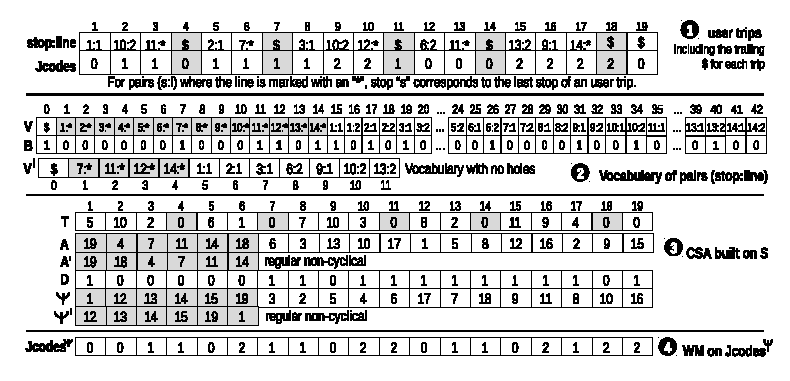
\includegraphics[width=1.00\textwidth]{ttctr2019.eps}
	%\vspace{-0.3cm}
	\caption{Structures involved in the creation of a \ttctr}
	\label{fig:ttctr}
	%\vspace{-0.2cm}
\end{figure}

After this, the sequence $T[1,n]$ is built, with the identifiers obtained from mapping mapping to the vocabulary entries of $V'$, over which a \texttt{CSA} is built, as seen in Figure~\ref{fig:ttctr}(3). Each encoded trip in $T$ is terminated with with additional $\$$ symbols. While in the final \texttt{CSA} we assign all these $\$$ a lexicographical value of 0 $(V[0])$, we assign them different values during the construction of the suffix array (A) to ensure that the entries for $\$$ in $A$ maintain the same order as in the original text. Finally, we make a modification on $\Psi$ to make the entries of each $\$$ point to the start of its own trip instead of the next one. These two modifications are proven necessary for our implemented queries, at the expense of losing some of the properties of a classic CSA. For reference, in Figure~\ref{fig:ttctr} we also present $A'$ and $\Psi'$, that show how our modifications compare to the original CSA.

The journey codes ($jcodes$) are encoded in $Jcodes^{\Psi}[1,n]$, as shown in Figure~\ref{fig:ttctr}(4), that is aligned to $\Psi$ instead of $T$. $Jcodes[8]= 1$ corresponds to $Jcodes^{\Psi}[14]=1$, since $A[14]=8$; $Jcodes[9]= 2$ corresponds to $Jcodes^{\Psi}[18]=2$, since $A[18]=9$; and so on. Recall that $jcodes$ are relative to their line identifiers, leading us to skip the $jcodes$ that would be aligned to the entries of $\Psi$ belonging to the final stops (represented as ``$s\!:\!*$" in $V$), as they lack line identifiers, which are in turn needed to identify a journey. Additionally, the first positions of $Jcodes^{\Psi}$, aligned with the $\$$ entries, we duplicate the same $jcodes$ as in the start of each trip.

%In parallel with the construction of $T$, we create a sequence $Jcodes[1,n]$ aligned to $T$ where we set, for each trip the $journey$-$id$ corresponding to each stage. Recall the $journey$-$id$ is the third term from the triples $(s_i,l_i,j_i),~i\in[1,k]$ from a trip. In addition, assuming that $s_p$ contains the $0$ corresponding to the terminator $\$$ for the trip, we set $Jcodes[p]\leftarrow j_1$ (i.e. the same journey-id as  the starting stop of the trip). According to the discussion above, Figure~\ref{fig:ttctr} shows:
%{\em (step-1)} the sequence of pairs $(stop,line)$ for each trip, and the corresponding $Jcodes$; {\em (step-2)} the vocabularies, including $V$, $B$, and $V'$ (ending stops $s$ of trips do not need the line, therefore we use ``$s\!:\!*$".);\footnote{In this example, with only $5$ trips,  we have only $11$ {\em used pairs} in $V$, but in a real scenario for each stop of each line ({\em existing pair} $(s,l)$) 
%	there will be a $1$ in $B$.} 
%and {\em (step-3)} the structures involved in the creation of \texttt{CSA} from which \ttctr~uses $\Psi$, $D$, (and $V'$, $B$).

%The temporal component of \ttctr includes the sequence $Jcodes$ described above. Recall $Jcodes$ contains $journey$-$ids$ aligned to the values in $T$, and that, for every line $l$ there are $n_j^l$ journeys sorted by their starting time and numbered as $0\dots n_j^l-1$, and also we have average accumulated times to reach each stop in the line. Therefore, this representation allows us to describe exact times for each stop.

% In practice, we use $Jcodes^{\Psi}$, which is aligned to $\Psi$ rather than to $T$. See in Figure~\ref{fig:ttctr}(4).
% Note that $Jcodes[8]= 1$ corresponds to $Jcodes^{\Psi}[14]=1$, since $A[14]=8$; 
%           $Jcodes[9]= 2$ corresponds to $Jcodes^{\Psi}[18]=2$, since $A[18]=9$; and so on.

Finally, $Jcodes^{\Psi}$ is represented with a \texttt{WM}, to support the operations we need to evaluate our proposed queries while avoiding the overhead of other types of indices that are not based in compact representations.

With \ttctr~we obtain a clear separation between the spatial representation of the trips (\texttt{CSA}) and the temporal representation (\texttt{WM} of $jcodes$), where the former can be used to address queries such as ``number of passengers that started their trip from a stop $X\in S$ and a line $l\in L$'' (\texttt{start\_X$_{L}$} from Section~\ref{sec:rq}) with a binary search of the pattern $\$,X_l$, while the later can be used to filter down these results to a time window (\texttt{start\_X$_{LT}$}) with a $range_{a,b}(S,i,j)$ operation over the \texttt{WM}, where $a$ and $b$ are $jcodes$ obtained from Algorithm~\ref{alg:jcodes} and $i$ and $j$ delimit the range of the results obtained in $\Psi$. Because the $\$$ symbols were made cyclical in $\Psi$, it is also possible to answer \texttt{from\_X\_to\_Y} queries by searching for a pattern $Y,\$,X_l$ instead.

\subsection{\ctr}
\label{sec:ctr}
A fundamental weakness of \ttctr~is that it requires several binary search operations over the \texttt{CSA} in the following cases:
\begin{itemize}
    \item We are interested in the number of passengers that started their trip at a stop $s$ and a time window $t_a...t_z$, but from \textbf{any line} (\texttt{start\_X$_{T}$} from Section~\ref{sec:rq}). As $jcodes$ are relative to lines, we must make a separate query for each possible $(X_{l_i}) \forall l_i \in L$ combination.
    \item We need to restrict the line of a final stop, in queries such as \texttt{end\_X$_{L}$} or \texttt{from\_X\_to\_Y$_{L}$} (and similar variations). Because the final stops belong to separate entries of the vocabulary that do not encode line identifiers, to restrict a stop $Y\in S$ to a line $l\in L$ we need to search for every possible expanded pattern $W_l,Y...$, for every stop $W$ from the line $l$ that could have been boarded before alighting at $Y$. While it looks tempting to address this issue by modifying the design of \ttctr~so that final stops also encode line identifiers, this would in turn make queries that do not restrict the line of the final stop inefficient, and we would need to perform a new query for every combination of $(s_{l_i}) \forall l_i \in L$, as in the previous case. \marginpar{\tiny Viendo los experimentos, uno se puede preguntar si no habria quedado mejor meter lineas en paradas finales...}
\end{itemize}

These weaknesses motivated us to develop a second version, \ctr, which reduces the complexity of the queries that restrict the final line, and delegates line checks on a new WM, allowing for more space-time trade-off. As in \ttctr, the input trips need to be sorted by the same criteria, but in \ctr~we use three complementary structures to represent each component of the sequence, as shown in Figure~\ref{fig:example_xctr}:
\begin{enumerate}[(i)]
    \item An adapted Compressed Suffix Array (\texttt{CSA}) over the stop identifiers of all trips, concatenated into a string with additional terminator symbols $\$$ appended at the end of each trip. As in the \texttt{CSA} from \ttctr, we make these $\$$ symbols maintain the order of the trips and cyclical in $\Psi$. Because this time we do not encode line and stop identifiers together and \texttt{CSA} only encodes stops, there is no need for a complex vocabulary anymore.
    \item \texttt{WML}: Aligned to the entries of (i) there is a Wavelet Matrix (WM) for the line identifiers of each stop. Aligned to the $\$$ section we duplicate the starting lines of each trip. As a trivial optimization, we build a separate WM for every stop, allowing us to save space due to the fact that a single stop does not usually belong to many lines, thus the average height of these WM is no larger (and usually smaller) than the height of a single WM.
    \item \texttt{WMJ}: A WM of jcodes aligned to the leaves of (ii). Note that this makes this structure dependant on (ii), which is coherent with the fact that journey codes themselves are relative to the line identifier. In case (ii) implements the optimization described, the entries of the WM must also be rearranged to match the delimited stops.
\end{enumerate}

\begin{figure}[hbt!]
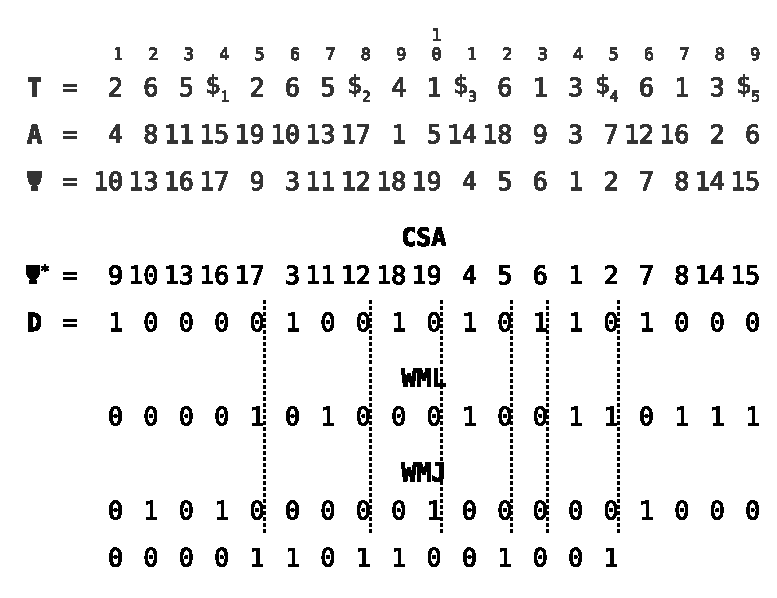
\includegraphics[width=\textwidth]{example_xctr.eps}
\caption{An example of five trips represented on \ctr~with the optimizations for \texttt{WML} and \texttt{WMJ}, and sections for each stop delimited by dotted lines}
\label{fig:example_xctr}
\end{figure}

As \ctr~is a complete representation of the collection of trips, we are able to extract any trip using the structures described. \marginpar{The idea here is that explaining how to extract will help understand the more complex FromXtoY query later} The algorithm to extract a trip is shown in the Algorithm~\ref{alg:extract}, where \FuncSty{Rank} and \FuncSty{Select} operate over the bitvector $D$ from our \texttt{CSA}, \FuncSty{WML}{(s$_a$)} is the WM corresponding to the stop \DataSty{s$_a$} in the optimized version of \texttt{WML} and \FuncSty{TrackDown} returns the leaf index of a WM given a root index. In a practical implementation, it is not needed to access \texttt{WML} and \texttt{WMJ} for the line identifier and jcode of the last stop of the trip, as they will always match the previous ones.

\begin{algorithm}[hbt!]
\SetKwData{la}{$l_a$}\SetKwData{lz}{$l_z$}\SetKwData{sa}{s$_a$}\SetKwData{sz}{s$_z$}\SetKwData{ta}{t$_a$}\SetKwData{tz}{t$_z$}\SetKwData{pattern}{pattern}\SetKwData{left}{left}\SetKwData{right}{right}\SetKwData{csa}{CSA}\SetKwData{wmj}{WMJ}\SetKwData{leftzero}{left$_0$}\SetKwData{rightzero}{right$_0$}\SetKwData{a}{a}\SetKwData{z}{z}\SetKwData{ja}{j$_a$}\SetKwData{jz}{j$_z$}\SetKwData{n}{n}\SetKwData{ap}{a'}\SetKwData{zp}{z'}\SetKwData{offset}{offset}\SetKwData{i}{i}\SetKwData{trip}{trip}
 \SetKwFunction{GetRange}{GetRange}\SetKwFunction{GetJCodes}{GetJCodes}\SetKwFunction{GetCount}{GetCount}\SetKwFunction{GetPsi}{$\Psi$}\SetKwFunction{GetRangeSpecial}{GetRange$^*$}\SetKwFunction{wml}{WML}\SetKwFunction{TrackUp}{TrackUp}\SetKwFunction{Select}{Select}\SetKwFunction{fxy}{FromXtoY\_full}\SetKwFunction{extract}{Extract\_trip}\SetKwFunction{access}{Access}\SetKwFunction{rank}{Rank}\SetKwFunction{TrackDown}{TrackDown}
 \SetKwProg{Fn}{Function}{\string:}{}
 
 \Fn{\extract{\i}}{
 \KwData{trip number \i}
 \KwResult{Sequence of tuples $<s,l,j>$ that compose the trip}
 \BlankLine
 \trip $\leftarrow$ []\;
 \a  $\leftarrow$ \GetPsi{\csa, \i}\;
 \sa $\leftarrow$ \rank{\csa,\a}\;
 \BlankLine
 \While{\sa $\neq$ 0}{
    \z $\leftarrow$ \Select{\csa,\sa}\;
    \la $\leftarrow$ \access{\wml{\sa}, \a-\z}\;
    \ja $\leftarrow$ \access{\wmj, \TrackDown{\wml{\sa}, \a-\z}+\z}\;
    append $<\sa,\la,\ja>$ to \trip\;
    \a  $\leftarrow$ \GetPsi{\csa, \i}\;
    \sa $\leftarrow$ \rank{\csa,\a}\;
 }
 \BlankLine
 \Return{\trip}\;
 }
 
 \caption{Extracting the trip \DataSty{i} from \ctr, where \FuncSty{CSA}, \FuncSty{WML} and \FuncSty{WMJ} are the structures previously described in (i), (ii) and (iii), respectively}
 \label{alg:extract}
\end{algorithm}

A more complex query that we can solve with \ctr~is ``number of trips that started from a stop \DataSty{s$_a$} and ended at a stop \DataSty{s$_z$}'', which can be further restricted to specific starting and ending lines and a time window (\texttt{from\_X$_{LT}$\_to\_Y$_{LT}$} in Section~\ref{sec:rq}). The pseudocode for the full version of such query can be found at the Algorithm~\ref{alg:xy}. This algorithm relies heavily on the abstract function \FuncSty{GetRange}, which when applied to a CSA, delimits the range of entries of $\Psi$ that match a queried string pattern, while on a WM it works as the $range$ operation defined in Section~\ref{sec:wm}, also reporting the range in the last level of a WM corresponding to the entries of a single queried symbol within a range in the encoded sequence (equivalent to two \FuncSty{TrackDown} operations on the first and last occurrence of the queried symbol, but more time efficient).

\begin{algorithm}[hbt!]
\SetKwData{la}{$l_a$}\SetKwData{lz}{$l_z$}\SetKwData{sa}{s$_a$}\SetKwData{sz}{s$_z$}\SetKwData{ta}{t$_a$}\SetKwData{tz}{t$_z$}\SetKwData{pattern}{pattern}\SetKwData{left}{left}\SetKwData{right}{right}\SetKwData{csa}{CSA}\SetKwData{wmj}{WMJ}\SetKwData{leftzero}{left$_0$}\SetKwData{rightzero}{right$_0$}\SetKwData{a}{a}\SetKwData{z}{z}\SetKwData{ja}{j$_a$}\SetKwData{jz}{j$_z$}\SetKwData{n}{n}\SetKwData{ap}{a'}\SetKwData{zp}{z'}\SetKwData{offset}{offset}
 \SetKwFunction{GetRange}{GetRange}\SetKwFunction{GetJCodes}{GetJCodes}\SetKwFunction{GetCount}{GetCount}\SetKwFunction{GetPsi}{$\Psi$}\SetKwFunction{GetRangeSpecial}{GetRange$^*$}\SetKwFunction{wml}{WML}\SetKwFunction{TrackUp}{TrackUp}\SetKwFunction{Select}{Select}\SetKwFunction{fxy}{FromXtoY\_full}
 \SetKwProg{Fn}{Function}{\string:}{}
 
 \Fn{\fxy{\la,\lz,\sa,\sz,\ta,\tz,\n}}{
 \KwData{lines \la,\lz, stops \sa,\sz, times \ta,\tz and length of the sequence \n}
 \KwResult{Number of occurences}
 \BlankLine
 \pattern $\leftarrow \{\sz,0,\sa\}$\;
 \left,\right $\leftarrow$ \GetRange{\csa, $0$, \n, \pattern}\;
 \leftzero $\leftarrow$ \GetPsi{\csa, \left}\;
 \rightzero $\leftarrow$ \GetPsi{\csa, \right}\;
 \tcp{\right-\left = \rightzero-\leftzero}
 \a,\z $\leftarrow$ \GetRange{\wml{$0$},\leftzero,\rightzero,\la}\;
 \ja,\jz $\leftarrow$ \GetJCodes{\la,\sa,\ta,\tz}\;
 \a,\z $\leftarrow$ \GetRangeSpecial{\wmj,\a,\z,\ja,\jz}\;
 \ap $\leftarrow$ \TrackUp{\wml{$0$},\a}\;
 \zp $\leftarrow$ \TrackUp{\wml{$0$},\z}\;
 \tcp{\z-\a = \zp-\ap}
 \offset $\leftarrow$ \Select{\csa,\sz}\;
 \a,\z $\leftarrow$ \GetRange{\wml{\sz},\left-\offset~$+$~\ap-\leftzero,
 \left-\offset~$+$~\zp-\leftzero,\lz}\;
 \ja,\jz $\leftarrow$ \GetJCodes{\lz,\sz,\ta,\tz}\;
 \Return{\GetCount{\wmj,\offset~+~\a,\offset~+~\z,\ja,\jz}}\;
 }
 
 \caption{Querying for all features on \ctr}
 \label{alg:xy}
\end{algorithm}

We will now proceed to explain the Algorithm~\ref{alg:xy} line by line:
\begin{itemize}
    \item In \textbf{lines 2-3}, we query our \FuncSty{CSA} for the pattern consisting of the destination stop \DataSty{s$_z$}, followed by a 0 (the code for the $\$$ symbol) and finally the origin stop \DataSty{s$_a$}. This results in a range of entries within the section of \DataSty{s$_z$} that belong to our queried trips, because the trips were made circular in $\Psi$, so each $\$$ points to the beginning of its own trip. If we were not interested in restricting lines nor time, the function would end here, returning \DataSty{right}-\DataSty{left}.
    
    \item In \textbf{lines 4-6} we obtain the corresponding range in the section of $\$$ by accessing \FuncSty{$\Psi$}. Note that because of how the sorting of the $\$$ symbols was altered during the construction of the suffix array, these two ranges are equal in size, as the comment in line 6 points out.
    
    \item In \textbf{line 7} we query \texttt{WML} in the $\$$ section, within the range previously obtained, for the queried starting line \DataSty{l$_a$}, obtaining the range of its occurrences in the last level, delimited by \DataSty{a} and \DataSty{z}. Note that if the \ctr~was constructed without the optimization that separates \texttt{WML} in sections, this line would be exactly the same, save for the query being on a \DataSty{WML} that would encode the whole sequence of lines instead of just the \DataSty{WML}{(0)} for $\$$.
    
    \item In \textbf{line 8} we obtain the range of jcodes for the journeys from the line \DataSty{l$_a$} that would pass through the stop \DataSty{s$_a$} within the time window delimited by \DataSty{t$_a$} and \DataSty{t$_z$}, using the function \FuncSty{GetJCodes} from Algorithm~\ref{alg:jcodes}.
    
    \item In \textbf{line 9} we operate over a range of \texttt{WMJ} that encodes a non-decreasing sequence of jcodes, given that within the same origin stop, final stop and starting line, the $\$$ were sorted by the starting journey code of their trips. This allows us to use a specially modified version of \FuncSty{GetRange} that is able to return the range of indexes on the first level of the WM instead of the last one. This is equivalent to finding the lower and upper bounds for the range \DataSty{j$_a$}$..$\DataSty{j$_z$} via binary searches in \FuncSty{WMJ} from \DataSty{a} to \DataSty{z}, but much more efficient.
    
    \item In \textbf{lines 10-12} we use the \FuncSty{TrackUp} operation, which is the inverse of \FuncSty{TrackDown}: it returns the root index given a leaf index of a WM. In this case, as the \FuncSty{a} and \FuncSty{z} we obtained in the previous step are also indexes in the last level of the \FuncSty{WML}, we use \FuncSty{TrackUp} to translate that range of indexes to the root of \texttt{WML} and therefore to the entries of the \texttt{CSA} as well. Note that this is a range inside the $\$$ section for trips with the same origin stop, final stop and starting line that includes all the trips for jcodes that span from \DataSty{j$_a$} to \DataSty{j$_z$}. The properties of our adapted \texttt{CSA} also ensure that this range maintains the same size after translation and it can also be directly translated to a range in the \DataSty{s$_z$}.
    
    \item In \textbf{line 13} we obtain the starting index of the section for the stop \DataSty{s$_z$} with a \FuncSty{Select} operation over the bitvector D from \texttt{CSA}. This is necessary for operating on \texttt{WML} and \texttt{WMJ} to restrict the line and journeys for the final stop.
    
    \item In \textbf{line 14} the range \DataSty{a'}$..$\DataSty{z'} is trivially translated to the section for \DataSty{s$_z$} where we query \texttt{WML} to obtain the subrange for the line \DataSty{l$_z$}. Remember that \DataSty{WML}{(s$_z$)} represents only the lines for \DataSty{s$_z$}, therefore both the translated indexes and the resulting subrange indexes are relative and must be adjusted by \DataSty{offset}. This would have not been necessary if the optimization was not implemented, and absolute indexes would have been used.
    
    \item In \textbf{line 15} we obtain the jcode range analogously to line 8, but this time for \DataSty{l$_z$} and \DataSty{s$_z$}.
    
    \item In \textbf{line 16} we return the number of entries of \texttt{WMJ} between \DataSty{j$_a$} and \DataSty{j$_z$} within our final subrange. The function \FuncSty{GetCount} does not report any range boundaries as \FuncSty{GetRange} does, but simply returns the number of occurrences. Of course, the time complexity of this operation is still proportional to the height of the WM.
    %even though the matching entries can be scattered (not delimiting a contiguous range).
\end{itemize}

It is trivial to reuse the Algorithm~\ref{alg:xy} to answer queries with less constrains. For example, if we were only interested in restricting the starting line, we could return \DataSty{z}-\DataSty{a} after line 7. Or if we only wanted to restrict the ending line and time, we can do it by skipping the lines 4-12, and using directly \FuncSty{GetRange}{(\FuncSty{WML}{(s$_z$)},left-offset,right-offset,l$_z$)} in line 14. The complexity would increase if we restricted by a time window but not by lines, as would need to iterate through all possible lines for \DataSty{s$_a$} and \DataSty{s$_z$} to obtain the jcodes for each line and perform these operations on \texttt{WML} and \texttt{WMJ}. Fortunately, the number of lines that a single stop can belong to tends to be rather small in practice, thus with a careful implementation that avoids repeating computation the performance of such query scales well, as will be shown later in Section~\ref{sec:exp}. Finally, to obtain only the trips that started on a given stop we would simply need to set \DataSty{pattern} to $\{0,s_a\}$ in line 2, or alternatively to $\{s_z,0\}$ for the final stop, and skipping the operations on the sections of \DataSty{s$_z$} or $\$$, respectively.

Of course, \ctr~can also be used to efficiently obtain other interesting information about trips, such as the top k most boarded stops, as shown in \cite{brisaboa2018compact}, with the additional possibility of differentiating stops that are only used to switch lines in \ctr. However, there is no known way of using this representation to obtain other kinds of information efficiently (e.g. the number of passengers in a journey between two stops).

\subsection{Comparing \acumm, \ttctr~and \ctr}
\label{sec:comp}
To illustrate the application of each representation, as well as highlight the motivation for the development of \ctr, we present in this section a comparison of worst case time complexities of each query described in Section~\ref{sec:rq}.

\begin{threeparttable}
\centering
\caption{Worst case time complexities of the representations in Section~\ref{sec:ps}}
\label{tab:queries}
\begin{tabular}{|l|l|l|l|}
\hline
Query &  \acumm & \ttctr & \ctr\\
\hline
\texttt{board\_X$_{LT}$} & $O(l)$\tnote{a} & $O(l\times \log(\bar{|J^l|}))$\tnote{abg} & \ctrq\tnote{b} \\
\texttt{alight\_X$_{LT}$} & $O(l)$\tnote{a} & Hard\tnote{cd} & Hard\tnote{cd} \\
\texttt{start\_X$_{LT}$} & - & \ttctrq\tnote{b} & \ctrq\tnote{b} \\
\texttt{end\_X$_{LT}$} & - & $O(|S|\times \ttctrq)$\tnote{be} & \ctrq\tnote{b} \\
\texttt{switch\_X$_{LT}$} & - & \ttctrq\tnote{b} & \ctrq\tnote{b} \\
\texttt{from\_X$_{LT}$\_to\_Y$_{LT}$} & - & $O(|S|\times \ttctrq)$\tnote{be} & \ctrq\tnote{b} \\
\texttt{board\_L$_T$} & O(1) & $O(|S|\times \log(\bar{|J^l|}))$\tnote{beg} & $O(|S| \times \ctrq)$\tnote{be} \\
\texttt{alight\_L$_T$} & O(1) & $O(|S|\times \log(\bar{|J^l|}))$\tnote{bceg} & $O(|S| \times \ctrq)$\tnote{bce} \\
\texttt{start\_L$_T$} & - & $O(|S|\times \ttctrq)$\tnote{be}~~~ & $O(\log(|L|\times\bar{|J^l|}))$\tnote{fg} \\
\texttt{end\_L$_T$} & - & Hard\tnote{d} & $O(|S| \times \ctrq)$\tnote{be} \\
\texttt{board\_T} & $O(|L|)$\tnote{f} & Hard\tnote{d} & Hard\tnote{d} \\
\texttt{alight\_T} & $O(|L|)$\tnote{f} & Hard\tnote{cd} & Hard\tnote{cd} \\
\texttt{start\_T} & - & Hard\tnote{d} & $O(|L| \times \log(|L|\times\bar{|J^l|}))$\tnote{fg}~~ \\
\texttt{end\_T} & - & Hard\tnote{d} & Hard\tnote{d} \\
\texttt{load\_X$_{LT}$} & $O(l)$\tnote{a} & Hard\tnote{cd} & Hard\tnote{cd} \\
\hline
\end{tabular}

\begin{tablenotes}
\item[a] $l$ is the number of lines we restrict to.
\item[b] The complexity of varies with the restrictions. See discussion.
\item[c] May include false positives.
\item[d] Not practical to solve with the indexing capabilities of this representation.
\item[e] $|S|$ is the number of stops in the line L.
\item[f] $|L|$ is the total number of lines represented.
\item[g] $\bar{|J^l|}$ is the average number of jcodes per line.
\end{tablenotes}
\end{threeparttable}

\medskip
Before explaining the details of how each of these operations would be implemented in our representations, it is worth noting that the complexity of \ctrq~will depend on the restrictions that are applied, as they will yield different variations of Algorithm~\ref{alg:xy}, as explained by the end of the Section~\ref{sec:ctr}. Generally, the time complexity of \ctrq~with all the restrictions is bounded by one \FuncSty{GetRange} operation on \FuncSty{CSA} to restrict by a stop id, one on \FuncSty{WML} to restrict by a line id and finally another one on \FuncSty{WMJ} to restrict by jcodes, with a total complexity of $O(\log(n\times|L|\times\bar{|J^l|}))$, being $n$ the size of the represented sequences\footnote{While theoretically locating a pattern of length $m$ in a Suffix Array takes $O(m \log n)$ time, in our case $m$ is bounded to 2 or 3 (in case of \texttt{from\_X\_to\_Y}). Furthermore, with a backward search implementation, only $m-1$ binary searches are needed.}.
However, when only the time is restricted, every line that the queried stop belongs to must be considered, thus increasing the worst-case complexity to $O(\log(n) + |L|\times \log(|L|\times\bar{|J^l|}))$. Similarly, the complexity of \ttctrq~is normally a search in the \texttt{CSA} and a \FuncSty{GetRange} on the \texttt{WM} (if time is restricted), which would amount to $O(\log(n) + \log(bar{|J^l|}))$, although when only the time and not the line is restricted, we must perform a new query for every possible line, and the complexity increases to $O(|L|\times (\log(n) + \log(bar{|J^l|})))$, which is generally higher than the one from \ctrq.

\begin{itemize}
    \item \texttt{board\_X$_{LT}$} This can be solved easily in the \acumm, as there are aggregated matrices for boarding stops, even though it is necessary to access a separate matrix for every line queried, hence $O(l)$. For \ttctr, the number of occurrences for the stop X is counted by delimiting its range on \FuncSty{D} (with a constant time $select$ operation) and filtering down the \texttt{WM} if needed. For \ctr, the filtering is done through \FuncSty{WML} and \FuncSty{WMJ}, and after that we must subtract the occurrences of final stops, obtained by one \texttt{end\_X$_{LT}$} with the same restrictions.
    \item \texttt{alight\_X$_{LT}$} Both in \ttctr~and \ctr, the only alighting stops that are explicitly represented are the final stops. To obtain an approximated count of the rest of them, we would need to extract and examine all the occurrences for \texttt{board\_W$_{LT}$} for every W that could have been boarded before X, as the worst-case time complexity of solving with their index operations is prohibitive. On the other hand, it can be solved much faster in \acumm~by accessing the alighting matrices.
    \item \texttt{start\_X$_{LT}$} Cannot be solved in \acumm. In the two other representations, we need to the range for the pattern $\$X$ in the \FuncSty{CSA} and filtering down \FuncSty{WML} and \FuncSty{WMJ} if needed.
    \item \texttt{end\_X$_{LT}$} In \ctr~it is solved similarly to \texttt{start\_X$_{LT}$}, by delimiting the range for the pattern $X\$$ in the \FuncSty{CSA} and filtering down \FuncSty{WML} and \FuncSty{WMJ} if needed. It can be much more complex for \ttctr, where the only way to restrict a line is to make a new query for every stop that could have been boarded before X in that line, which is a problem detailed at the start of Section~\ref{sec:ctr}.
    \item \texttt{switch\_X$_{LT}$} Calculated as board\_X$_{LT}$ - start\_X$_{LT}$.
    \item \texttt{from\_X$_{LT}$\_to\_Y$_{LT}$} Explained in detail in Algorithm~\ref{alg:xy}. In \ttctr~the $|S|$ factor only takes effect if the line (or time) for Y must be restricted, as for \texttt{end\_X$_{LT}$}.
    \item \texttt{board\_L$_T$} Straightforward in \acumm, as it only needs to access one matrix. For \ttctr~we must filter through the \texttt{WM} for every stop from L. While in \ctr~the total number of occurrences of line L can be calculated in one $O(\log|L|)$ operation (with additional filtering through \FuncSty{WMJ} if needed), we need to subtract the occurrences of start\_L$_T$ and end\_L$_T$, the later having a greater complexity of $O(|S| \times \ctrq)$.
    \item \texttt{alight\_L$_T$} Can be approximated both in \ttctr~and \ctr~with board\_L$_T$, given that every user that boards on a line is expected to alight from it within a reasonable time.
    \item \texttt{start\_L$_T$} Trivially solved in \ctr, by filtering down \FuncSty{WML} and \FuncSty{WMJ}, if needed, over the $\$$ section of the \FuncSty{CSA}. On the other hand, for \ttctr~the \texttt{CSA} needs to be queried with the $\$X$ pattern for every stop X from line $l$.
    \item \texttt{end\_L$_T$} Can be solved in \ctr, by performing a end\_X$_{LT}$ for every stop X from the line $l$. If we did the same for \ttctr, we would end up with a complexity of $O(|S|^2\times\ttctrq)$, which we consider prohibitive.
    \item \texttt{board\_T} and \texttt{alight\_T} Although \acumm, \ttctr~and \ctr~could solve it by applying board\_L$_T$ $|L|$ times, this would imply a prohibitive cost for both \ttctr~and \ctr, where extracting all the trips would be preferred in practice.
    \item \texttt{start\_T} Solved in the \ctr~by applying \texttt{start\_X$_{LT}$} $|L|$ times.
    \item \texttt{end\_T} None of our representations can solve this query efficiently, although it could be approximated by \texttt{start\_T} in CTR.
    \item \texttt{load\_X$_{LT}$} This can be easily calculated in \acumm~as detailed in Section~\ref{sec:acumm}. \marginpar{Tirso please explain how!}
\end{itemize}

\section{Experiments}
\label{sec:exp}
In this section we discuss the practical performance of our structures. To evaluate them, we have run randomly generated queries against \acumm, \ttctr~and \ctr~built over a dataset of user trips over a real transportation network (Section~\ref{sec:data}), with several configurations to study the trade-off between compression (Section~\ref{sec:space}) and query efficiency (Section~\ref{sec:time}), and testing different configurations for each individual structure.

\subsection{Experimental dataset}
\label{sec:data}
Using real GTFS\footnote{\url{https://developers.google.com/transit/gtfs/}} descriptions of bus routes and schedules, we generated a synthetic dataset of user trips that aims to realistically imitate real user behaviour over a month. In this work, we have combined the GTFS obtained for the networks of urban\footnote{Provided by EMT \url{http://www.emtmadrid.es}} and interurban\footnote{Provided by CRTM \url{http://www.crtm.es}} buses for the city of Madrid. The network model is extracted and user trips are generated with the following general steps:

\begin{enumerate}
    \item Parse stop, route and trip identifiers. This usually produces two lines per route, one for each direction. With this we are able to build the common structures $lineStop$ and $stopLine$.
    \item Connect stops that are on a short walking distance (100 meters) from each other, or appear sequentially on the same line.
    \item Parse the schedules for bus trips.
    \item Generate a month of journeys from the schedules, differentiating days of week. From this we compute $avgTime$ and $initialTime$.
    \item Generate user trips. A trip starts from a random stop, day and journey and simulates boarding that journey and traversing it. After each traversed stop, the user may end the trip with a probability that starts at zero and increases by 1\% for every stop visited. Additionally, there is a fixed probability of attempting to switch lines at the current stop, if there is a journey available at that stop within the allowed waiting time (30 minutes) and from a different line\footnote{The reverse of the current line is also disallowed.}. Switching lines is also attempted when the end of the current line is reached.
    \item We persist these generated trips as sequences of stages \\ $<<line,journey,boarding\_stop>, <line,journey,alighting\_stop>>$,\\ where a boarding and alighting stop naturally share the same line and journey within the same stage. This results in the same number of stages as lines have been used. With the parameters used, about 56\% of our trips have one stage, 33\% have two, 9\% have three and 2\% have four.
\end{enumerate}

With this approach we have generated a dataset of ten million trips, over a real network consisting of 11021 stops, 1048 lines for a simulated month\footnote{A period of 31 days, starting with a Monday.}, with an average of 1622 journeys per line and a maximum of 9980. We consider that this synthetic dataset is of enough accuracy and size to obtain significant results when studying the compression capabilities and performance of our representations.

\subsection{Space requirements}
\label{sec:space}
We have measured the sizes of all the individual components of our representation in memory when built over the experimental dataset. We present the sizes of our common structures, followed by the \acumm\marginpar{Missing \acumm~sizes!}. After that, we compare the compression achieved with \ttctr~and \ctr.

For the \texttt{CSA} structures from \ttctr~and \ctr, we experiment with the $t_\Psi$ (sampling interval) factors of 32, 128 and 512. For the \texttt{WM} present in \ttctr, as well as in the two \texttt{WM} from \ctr, we analyze the compression achieved with the \texttt{RRR} bitvector described in \cite{Raman:2002:SID:545381.545411}, using block sizes of 32, 64 and 128, and compare it against a plain bitvector with a rank structure, which we call \texttt{RG32}. \marginpar{\tiny Do we have any similar trade-off for \acumm?}

The space occupied by the common structures is reflected in Table~\ref{tab:commons}. These were represented using plain fixed bit length integers with the exception of $initialTime$, where we used the compression approach discussed in Section~\ref{sec:cs} with a sampling interval of 512. This has allowed us to represent all required network information in a negligible space of less than 1 MiB.

\begin{table}
    \centering
    \caption{Sizes of the common structures}
    \label{tab:commons}
    \begin{tabular}{|c|c|c|c|c|c|}
    \hline
        Structure & $lineStop$ & $stopLine$ & $avgTime$ & $initialTime$ & Total \\
        \hline
        Size (KiB) & 119 & 141 & 64 & 440 & 764 \\
    \hline
    \end{tabular}
\end{table}

In Table~\ref{tab:ttctr} we analyze the space occupied by the two structures of \ttctr: a \texttt{CSA} that encodes stops and their lines, and a \texttt{WM} that encodes journey codes.

\begin{table}
    \caption{Space requirements for the \texttt{CSA} (a) and the \texttt{WM} (b) from \ttctr}
    \label{tab:ttctr}
    \begin{subtable}[t]{.48\linewidth}
    \vspace{-12pt}
    \caption{\footnotesize (a)}
    \vspace{-12pt}
    \begin{tabular}[t]{|l|l|r|r|}
        \hline
        t$_\Psi$ & bps & Size (MiB) & Comp. (\%) \\
         \hline
        baseline & 16 & 67.85 & 100.00 \\
        32 & 7.288 & 30.91 & 45.55 \\
        128 & 6.069 & 25.74 & 37.93 \\
        512 & 5.761 & 24.43 & 36.01 \\
        \hline
    \end{tabular}
    \end{subtable}%
    \begin{subtable}[t]{.48\linewidth}
    \vspace{-12pt}
    \caption{\footnotesize (b)}
    \vspace{-12pt}
    \begin{tabular}[t]{|l|l|r|r|}
        \hline
        Bitvector & bps & Size (MiB) & Comp. (\%) \\
         \hline
        baseline & 14 & 42.68 & 100.00 \\
        RG32 & 14.438 & 44.02 & 103.13 \\
        RRR32 & 13.478 & 41.09 & 96.27 \\
        RRR64 & 12.79 & 38.99 & 91.36 \\
        RRR128 & 12.446 & 37.94 & 88.90 \\
        \hline
    \end{tabular}
    \end{subtable}
\end{table}

The baseline used for the \texttt{CSA} is a plain representation of the sequence encoded by the \texttt{CSA}, omitting the cost of a dictionary to filter nonexistent combinations of lines and stops. Even when compared to this compact baseline, the \texttt{CSA} is able to achieve remarkable compression rates, as it captures the repetitiveness of trips when constrained to our network of bus lines.

We were not able to achieve such compression rates for the \texttt{WM}, where compressing the bitvectors with \texttt{RRR} results in a \texttt{WM} that is only slightly smaller than the baseline plain representation of all journey codes. This sequence is indeed hard to compress, given than it was rearranged to be aligned to the entries of our \texttt{CSA}, which nullifies any local redundancy that other kinds of arrangements may obtain.

We also measured the occupied space of \ctr~in Table~\ref{tab:ctr}, where three structures must be taken in consideration: a \texttt{CSA} that only encodes stop identifiers, and two \texttt{WM}: one for line identifiers (\texttt{WML}) and one for journey codes (\texttt{WMJ}).

\begin{table}
    \caption{Space requirements for the \texttt{CSA} (a), the \texttt{WMJ} (b) and the \texttt{WML} (c) from \ctr}
    \label{tab:ctr}
    \begin{subtable}[t]{.48\linewidth}
    \vspace{-12pt}
    \caption{\footnotesize (a)}
    \vspace{-12pt}
    \begin{tabular}[t]{|l|l|r|r|}
        \hline
        t$_\Psi$ & bps & Size (MiB) & Comp. (\%) \\
         \hline
        baseline & 14 & 59.37 & 100.00 \\
        32 & 6.956 & 29.50 & 49.69 \\
        128 & 5.727 & 24.29 & 40.91 \\
        512 & 5.417 & 22.97 & 38.69 \\
        \hline
    \end{tabular}
    \end{subtable}
    \begin{subtable}[t]{.48\linewidth}
    \vspace{-12pt}
    \caption{\footnotesize (b)}
    \vspace{-12pt}
    \begin{tabular}[t]{|l|l|r|r|}
        \hline
        Bitvector & bps & Size (MiB) & Comp. (\%) \\
         \hline
        baseline & 14 & 59.37 & 100.00 \\
        RG32 & 14.438 & 61.23 & 103.13 \\
        RRR32 & 13.419 & 56.91 & 95.85 \\
        RRR64 & 12.732 & 53.99 & 90.94 \\
        RRR128 & 12.388 & 52.53 & 88.49 \\
        \hline
    \end{tabular}
    \end{subtable}
    \begin{subtable}[t]{.48\linewidth}
    \vspace{-12pt}
    \caption{\footnotesize (c)}
    \vspace{-12pt}
    \begin{tabular}[t]{|l|l|r|r|}
        \hline
        Bitvector & bps & Size (MiB) & Comp. (\%) \\
         \hline
        baseline & 11 & 46.65 & 100.00 \\
        RG32 & 4.778 & 20.26 & 43.44 \\
        RG32 & 2.338 & 9.91 & 21.25 \\
        RG64 & 2.18 & 9.24 & 19.82 \\
        RG128 & 2.103 & 8.92 & 19.12 \\
        \hline
    \end{tabular}
    \end{subtable}%
\end{table}

When comparing to the structures of \ttctr, we can observe that \texttt{WMJ} of \ctr, despite achieving a marginally better compression than the \texttt{WM} from \ttctr, requires considerably more space, as the sequence of jcodes from \ctr~includes final stops, while in \ttctr~they are skipped.

Although the \texttt{CSA} is slightly smaller in \ctr, the compression ratios are worse than the ones in \ttctr~when we compare to a smaller baseline that only represents the sequence of stops, with no information about lines. Even at the sparsest sample rate of 512, the compression ratio of the \texttt{CSA} in \ctr~is worse than the ratio achieved in \ttctr~with a sample rate of 128.

This difference is accentuated when we consider that we must add the space of \texttt{WML} to \ctr, even though we obtain much better compression than for \texttt{WMJ}. The compression observed with the uncompressed bitvector \texttt{RG32} is due to the optimization discussed in Section~\ref{sec:ctr}, where we keep a separate \texttt{WM} aligned to each stop from the \texttt{CSA}, resulting in much shorter \texttt{WM}s. The further compression achieved with the \texttt{RRR} bitvectors is possible because the stop entries in the \texttt{CSA} are sorted by either the final stop the user alights to or the next stop to board, making the aligned sequence of lines very predictable. Additionally, as our \texttt{CSA} maintains the order of trips from the original text in the $\$$ section, leading to the formation of clusters in the first \texttt{WML}.

\subsection{Query performance}
\label{sec:time}
Missing a comparison of \acumm~vs \ttctr!

We have implemented the most adequate queries for \ttctr~and \ctr~from those described in Section~\ref{sec:rq}, and measured their average execution time from 100.000 randomly generated queries on [rellenar detalles de Compostela 2]. In this section we will only discuss four of the possible configurations tested for both \ttctr~and \ctr, with t$_{\Psi}$ values of 32 and 512 combining with WM using either uncompressed bitvectors (\texttt{RG32}) or the most compressed (\texttt{RRR128})\footnote{In case of \ctr, this refers to bitvectors from both \texttt{WML} and \texttt{WMJ}.}. These four configurations should be illustrative enough to provide an understanding of the space-time trade-offs of our approaches, although the execution times for all tested configurations can be found in the Appendix A.

We demonstrate the main advantage of \ctr~over the older \ttctr~ in the Figure~\ref{fig:start}b, where restricting a line or a time interval for an \texttt{end\_X} query is very expensive for \ttctr~ due to its separate vocabulary for final stops, requiring to query the \texttt{CSA} for every possible stop that could have been boarded before X to restrict a line. In the Figure~\ref{fig:start}a it is also possible to see how the performance of \ctr~degrades less with a highly compressed \texttt{CSA} for the query \texttt{start\_X$_T$}, where even queries over a compressed \texttt{WML} are faster than queries over the \texttt{CSA}.

\marginpar{Consider changing the order of the bars}

\begin{figure}[hbt!]
\begin{subfigure}{0.5\linewidth}
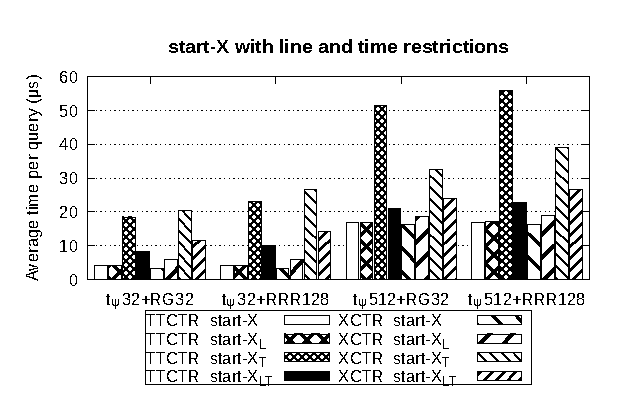
\includegraphics[width=\linewidth]{experiments/start.eps}
\vspace{-12pt}
\caption{\footnotesize (a)}
\vspace{-12pt}
\end{subfigure}%
\begin{subfigure}{0.5\linewidth}
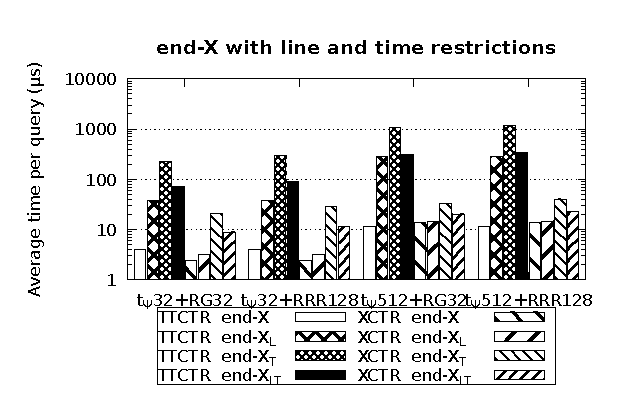
\includegraphics[width=\linewidth]{experiments/end.eps}
\vspace{-12pt}
\caption{\footnotesize (b)}
\vspace{-12pt}
\end{subfigure}
\caption{Comparison of \texttt{start\_X$_{LT}$} (a) and \texttt{end\_X$_{LT}$} (b) queries, with all variants. Note the logarithmic scale for the y axis in (b)}
\label{fig:start}
\end{figure}

Remember that restricting both the line and time is always cheaper than only restricting the time, as for the later more operations need to be performed to filter every line. This explains why $T$ queries are always slower than $LT$ queries. This is true for both representations, with any configuration and query.

We can see more examples of this difference in performance between these two representations with the \texttt{from\_X\_to\_Y} queries in the Figure~\ref{fig:xy0}, whenever the end lines or times are restricted. Additionally, we can yet again observe how using the most sparse sampling of $\Psi$ affects much more the \ttctr~than the \ctr, with the performance of \texttt{from\_X$_{T}$\_to\_Y} consistent with the \texttt{start\_X$_T$} shown in Figure~\ref{fig:start}a.

\begin{figure}[hbt!]
\begin{subfigure}{0.5\linewidth}
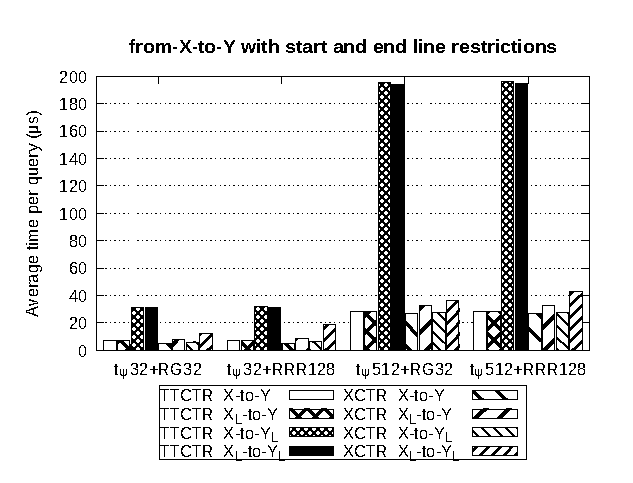
\includegraphics[width=\linewidth]{experiments/xy0.eps}
\vspace{-12pt}
\caption{\footnotesize (a)}
\vspace{-12pt}
\end{subfigure}%
\begin{subfigure}{0.5\linewidth}
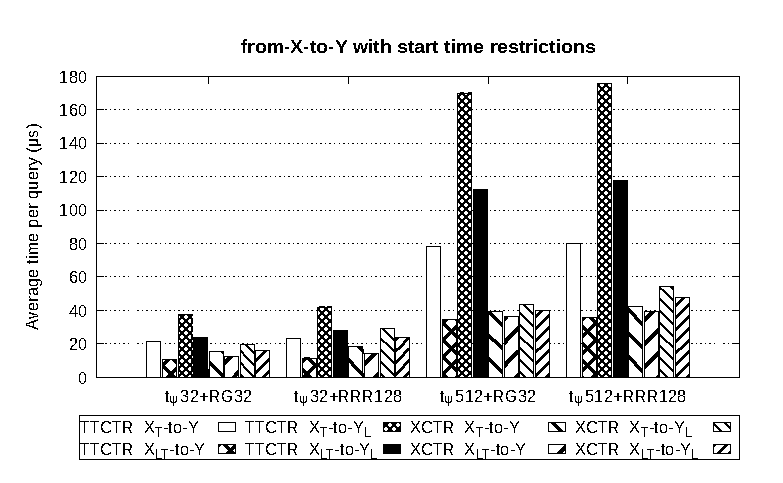
\includegraphics[width=\linewidth]{experiments/xy1.eps}
\vspace{-12pt}
\caption{\footnotesize (b)}
\vspace{-12pt}
\end{subfigure}
\caption{Comparison of \texttt{from\_X$_{LT}$\_to\_Y$_{LT}$} queries, variating line (a) and starting time (b) restrictions}
\label{fig:xy0}
\end{figure}

The performance of both representations can sometimes improve  when more selective restrictions are added, where the execution is cut short when no matching trips are found, before evaluating further restrictions. For this reason, the average times for \texttt{from\_X$_{T}$\_to\_Y$_{L}$} and \texttt{from\_X$_{LT}$\_to\_Y$_{L}$} are shorter than those of \texttt{from\_X\_to\_Y$_{L}$} and \texttt{from\_X$_{L}$\_to\_Y$_{L}$}.

When restricting to the end time, \ctr~consistently outperforms \ttctr, as shown in the Figure~\ref{fig:xy2}. which is to be expected considering the large number of times that the \texttt{CSA} from \ttctr~needs to be queried, yielding results similar to those from the Figure~\ref{fig:start}b where the end time is also restricted.

\begin{figure}[hbt!]
\begin{subfigure}{0.5\linewidth}
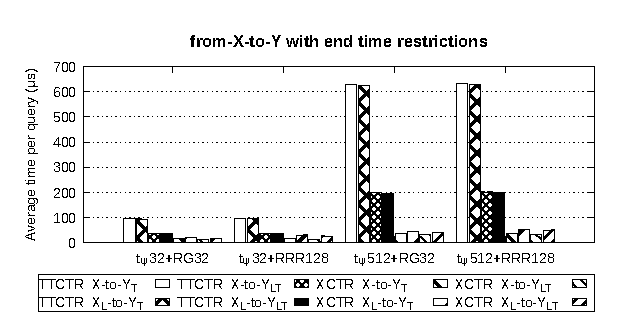
\includegraphics[width=\linewidth]{experiments/xy2.eps}
\vspace{-12pt}
\caption{\footnotesize (a)}
\vspace{-12pt}
\end{subfigure}%
\begin{subfigure}{0.5\linewidth}
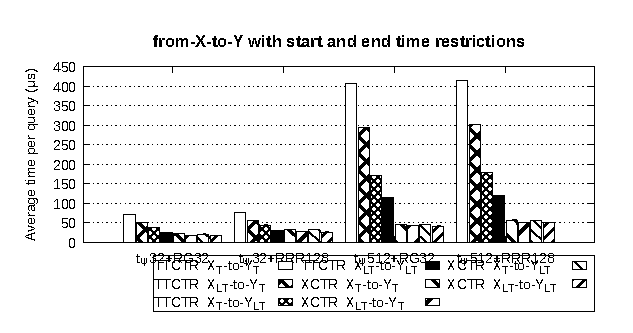
\includegraphics[width=\linewidth]{experiments/xy3.eps}
\vspace{-12pt}
\caption{\footnotesize (b)}
\vspace{-12pt}
\end{subfigure}
\caption{Comparison of \texttt{from\_X$_{LT}$\_to\_Y$_{LT}$} queries, variating line (a) and starting time (b) restrictions with a fixed ending time restriction}
\label{fig:xy2}
\end{figure}

The high selectivity of time restrictions explain why \ttctr~appears to become more competitive with the most restrictive queries of Figure~\ref{fig:xy2}b. However, its query time still increases several times when the \texttt{CSA} is highly compressed.

The only query for which \ttctr~is clearly preferred over \ctr~is \texttt{board\_X}, with any restriction, as can be seen in the Figure~\ref{fig:board}. Both for \texttt{board\_X} and \texttt{board\_X$_{L}$}, \ttctr~takes on average less than one microsecond per query, as the only operations needed are two constant time $select$ over the bitvector \texttt{D} from the \texttt{CSA}, while \ctr~needs to subtract the occurrences of $X\$$ (as those are alighting stops, not boarding), for which $\Psi$ must be accessed. This advantage is carried on the queries with time restrictions as well. \marginpar{\tiny Meter otra grafica aqui comparando tiempos de \ttctr~vs \acumm~para esta query}.

\begin{figure}[hbt!]
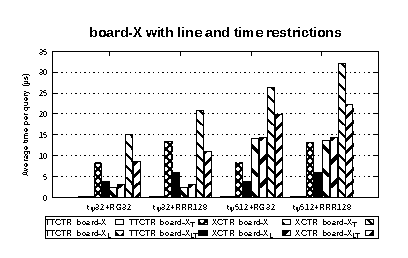
\includegraphics[width=0.5\textwidth]{experiments/board.eps}
\caption{Comparison of \texttt{board\_X$_{LT}$} queries, with all variants}
\label{fig:board}
\end{figure}

\section{Conclusions}
Speak about how cool would it be to have a single structure that could to it all. Pitch for our next paper with Gonzalo!

%
% ---- Bibliography ----
%
% BibTeX users should specify bibliography style 'splncs04'.
% References will then be sorted and formatted in the correct style.

\bibliographystyle{splncs04}
\bibliography{refs}

\appendix
\chapter*{Appendix A: Execution time for all tested configurations}
\label{app:times}
The following are the the average execution times from 100.000 randomly generated queries of each type on an Intel Xeon E5-2620v4@2.1 GHz machine. All results are in $\mu$sec.

%\section{Execution times on \ttctr}

\begin{table}[hpt!]
\caption{Execution times of \texttt{board\_X$_{LT}$} queries for \ttctr, with all variants.}
\begin{tabular}{|r|r|r|r|r|r|r|}
\hline
$t_{\Psi}$ & \texttt{WM} & \texttt{board\_X} & \texttt{board\_X$_{L}$} & \texttt{board\_X$_{T}$} & \texttt{board\_X$_{LT}$} \\
\hline
32 & RG32 & 0.17 & 0.12 & 8.21 & 3.87 \\
32 & RRR32 & 0.17 & 0.12 & 10.92 & 5.14 \\
32 & RRR64 & 0.17 & 0.13 & 11.71 & 5.35 \\
32 & RRR128 & 0.17 & 0.13 & 13.35 & 5.99 \\
128 & RG32 & 0.17 & 0.13 & 8.24 & 3.88 \\
128 & RRR32 & 0.17 & 0.13 & 10.90 & 5.12 \\
128 & RRR64 & 0.17 & 0.12 & 11.67 & 5.36 \\
128 & RRR128 & 0.17 & 0.13 & 13.19 & 5.92 \\
512 & RG32 & 0.17 & 0.13 & 8.22 & 3.86 \\
512 & RRR32 & 0.17 & 0.12 & 10.90 & 5.12 \\
512 & RRR64 & 0.17 & 0.13 & 11.64 & 5.41 \\
512 & RRR128 & 0.17 & 0.13 & 13.22 & 5.95 \\
\hline
\end{tabular}
\end{table}

\begin{table}[hpt!]
\caption{Execution times of \texttt{start\_X$_{LT}$} queries for \ttctr, with all variants.}
\begin{tabular}{|r|r|r|r|r|r|r|}
\hline
$t_{\Psi}$ & \texttt{WM} & \texttt{start\_X} & \texttt{start\_X$_{L}$} & \texttt{start\_X$_{T}$} & \texttt{start\_X$_{LT}$} \\
\hline
32 & RG32 & 4.20 & 4.16 & 18.52 & 8.22 \\
32 & RRR32 & 4.18 & 4.18 & 21.01 & 9.43 \\
32 & RRR64 & 4.21 & 4.15 & 21.70 & 9.65 \\
32 & RRR128 & 4.18 & 4.15 & 23.20 & 10.22 \\
128 & RG32 & 6.96 & 6.94 & 25.05 & 10.68 \\
128 & RRR32 & 6.96 & 6.94 & 27.44 & 11.78 \\
128 & RRR64 & 6.95 & 6.95 & 28.05 & 12.04 \\
128 & RRR128 & 6.94 & 6.94 & 29.64 & 12.62 \\
512 & RG32 & 17.01 & 16.85 & 51.36 & 21.13 \\
512 & RRR32 & 17.03 & 16.92 & 53.78 & 21.80 \\
512 & RRR64 & 17.05 & 16.86 & 54.43 & 22.01 \\
512 & RRR128 & 17.00 & 17.08 & 55.88 & 22.65 \\
\hline
\end{tabular}
\end{table}

\begin{table}[hpt!]
\caption{Execution times of \texttt{end\_X$_{LT}$} queries for \ttctr, with all variants.}
\begin{tabular}{|r|r|r|r|r|r|r|}
\hline
$t_{\Psi}$ & \texttt{WM} & \texttt{end\_X} & \texttt{end\_X$_{L}$} & \texttt{end\_X$_{T}$} & \texttt{end\_X$_{LT}$} \\
\hline
32 & RG32 & 1.41 & 35.26 & 224.45 & 68.07 \\
32 & RRR32 & 1.40 & 35.08 & 251.63 & 77.05 \\
32 & RRR64 & 1.40 & 35.24 & 263.88 & 80.63 \\
32 & RRR128 & 1.40 & 35.12 & 288.41 & 88.33 \\
128 & RG32 & 1.40 & 83.96 & 412.51 & 116.58 \\
128 & RRR32 & 1.42 & 84.11 & 439.37 & 125.26 \\
128 & RRR64 & 1.41 & 84.04 & 452.08 & 129.07 \\
128 & RRR128 & 1.40 & 84.09 & 477.22 & 137.03 \\
512 & RG32 & 1.41 & 272.22 & 1078.30 & 305.42 \\
512 & RRR32 & 1.43 & 272.47 & 1109.32 & 314.62 \\
512 & RRR64 & 1.41 & 272.19 & 1119.29 & 318.13 \\
512 & RRR128 & 1.40 & 272.53 & 1146.49 & 325.90 \\
\hline
\end{tabular}
\end{table}

\begin{table}[hbpt!]
\caption{Execution times of \texttt{from\_X\_to\_Y} queries for \ttctr, variating start and end line restrictions.}
\begin{tabular}{|r|r|r|r|r|r|r|}
\hline
$t_{\Psi}$ & \texttt{WM} & \texttt{from\_X\_to\_Y} & \texttt{from\_X$_{L}$\_to\_Y} & \texttt{from\_X\_to\_Y$_{L}$} & \texttt{from\_X$_{L}$\_to\_Y$_{L}$} \\
\hline
32 & RG32 & 7.11 & 7.10 & 31.24 & 31.03 \\
32 & RRR32 & 7.13 & 7.11 & 31.24 & 31.02 \\
32 & RRR64 & 7.15 & 7.14 & 31.20 & 31.00 \\
32 & RRR128 & 7.15 & 7.10 & 32.14 & 31.05 \\
128 & RG32 & 11.62 & 11.59 & 65.07 & 64.60 \\
128 & RRR32 & 11.66 & 11.59 & 65.16 & 64.72 \\
128 & RRR64 & 11.62 & 11.59 & 65.13 & 65.45 \\
128 & RRR128 & 11.62 & 11.58 & 65.10 & 64.66 \\
512 & RG32 & 28.37 & 28.22 & 195.18 & 193.64 \\
512 & RRR32 & 28.37 & 28.21 & 195.99 & 194.62 \\
512 & RRR64 & 28.37 & 28.21 & 196.03 & 194.40 \\
512 & RRR128 & 28.40 & 28.24 & 195.88 & 194.33 \\
\hline
\end{tabular}
\end{table}

\begin{table}[hbpt!]
\caption{Execution times of \texttt{from\_X$_T$\_to\_Y} queries for \ttctr, with starting time restrictions and variating start and end line restrictions.}
\begin{tabular}{|r|r|r|r|r|r|r|}
\hline
$t_{\Psi}$ & \texttt{WM} & \texttt{from\_X$_{T}$\_to\_Y} & \texttt{from\_X$_{LT}$\_to\_Y} & \texttt{from\_X$_{T}$\_to\_Y$_{L}$} & \texttt{from\_X$_{LT}$\_to\_Y$_{L}$} \\
\hline
32 & RG32 & 21.37 & 10.38 & 37.27 & 23.88 \\
32 & RRR32 & 22.25 & 11.05 & 39.45 & 25.74 \\
32 & RRR64 & 22.46 & 11.17 & 40.14 & 26.40 \\
32 & RRR128 & 22.98 & 11.57 & 42.00 & 27.89 \\
128 & RG32 & 32.83 & 15.25 & 64.04 & 41.68 \\
128 & RRR32 & 33.91 & 15.89 & 66.38 & 43.77 \\
128 & RRR64 & 33.90 & 16.04 & 67.09 & 44.20 \\
128 & RRR128 & 34.41 & 16.37 & 68.93 & 45.71 \\
512 & RG32 & 78.45 & 34.57 & 169.98 & 112.46 \\
512 & RRR32 & 79.33 & 35.25 & 172.87 & 114.77 \\
512 & RRR64 & 79.56 & 35.39 & 173.66 & 115.51 \\
512 & RRR128 & 80.11 & 35.75 & 175.46 & 117.63 \\
\hline
\end{tabular}
\end{table}

\begin{table}[hbpt!]
\caption{Execution times of \texttt{from\_X\_to\_Y$_T$} queries for \ttctr, with ending time restrictions and variating start and end line restrictions.}
\begin{tabular}{|r|r|r|r|r|r|r|}
\hline
$t_{\Psi}$ & \texttt{WM} & \texttt{from\_X\_to\_Y$_{T}$} & \texttt{from\_X$_{L}$\_to\_Y$_{T}$} & \texttt{from\_X\_to\_Y$_{LT}$} & \texttt{from\_X$_{L}$\_to\_Y$_{LT}$} \\
\hline
32 & RG32 & 94.47 & 93.05 & 34.71 & 34.11 \\
32 & RRR32 & 96.03 & 94.39 & 35.59 & 35.01 \\
32 & RRR64 & 96.79 & 94.70 & 35.86 & 35.18 \\
32 & RRR128 & 97.06 & 95.37 & 36.20 & 35.60 \\
128 & RG32 & 214.77 & 212.42 & 68.32 & 67.44 \\
128 & RRR32 & 216.61 & 214.44 & 69.40 & 68.54 \\
128 & RRR64 & 216.64 & 214.10 & 69.49 & 68.59 \\
128 & RRR128 & 218.35 & 214.48 & 69.78 & 69.12 \\
512 & RG32 & 630.29 & 625.12 & 198.43 & 196.33 \\
512 & RRR32 & 634.07 & 628.69 & 199.82 & 198.00 \\
512 & RRR64 & 634.95 & 629.76 & 200.36 & 198.32 \\
512 & RRR128 & 635.32 & 629.63 & 200.56 & 198.51 \\
\hline
\end{tabular}
\end{table}

\begin{table}[hbpt!]
\caption{Execution times of \texttt{from\_X$_T$\_to\_Y$_T$} queries for \ttctr, with starting and ending time restrictions and variating start and end line restrictions.}
\begin{tabular}{|r|r|r|r|r|r|r|}
\hline
$t_{\Psi}$ & \texttt{WM} & \texttt{from\_X$_{T}$\_to\_Y$_{T}$} & \texttt{from\_X$_{LT}$\_to\_Y$_{T}$} & \texttt{from\_X$_{T}$\_to\_Y$_{LT}$} & \texttt{from\_X$_{LT}$\_to\_Y$_{LT}$} \\
\hline
32 & RG32 & 71.26 & 50.47 & 38.48 & 25.16 \\
32 & RRR32 & 74.36 & 53.03 & 41.26 & 27.62 \\
32 & RRR64 & 75.19 & 53.69 & 42.18 & 28.20 \\
32 & RRR128 & 77.22 & 55.41 & 44.20 & 29.91 \\
128 & RG32 & 145.78 & 104.37 & 65.36 & 42.97 \\
128 & RRR32 & 149.11 & 107.27 & 68.34 & 45.37 \\
128 & RRR64 & 150.74 & 107.69 & 69.01 & 46.03 \\
128 & RRR128 & 151.66 & 109.30 & 71.09 & 47.69 \\
512 & RG32 & 408.12 & 294.89 & 171.26 & 113.68 \\
512 & RRR32 & 412.73 & 298.64 & 174.72 & 116.46 \\
512 & RRR64 & 413.86 & 299.46 & 175.60 & 117.25 \\
512 & RRR128 & 415.60 & 300.92 & 177.78 & 118.79 \\
\hline
\end{tabular}
\end{table}

%\section{Execution times on \ctr}

\begin{table}
\caption{Execution times of \texttt{board\_X$_{LT}$} queries for \ctr, with all variants.}
\begin{tabular}{|r|r|r|r|r|r|r|}
\hline
$t_{\Psi}$ & \texttt{WML} & \texttt{WMJ} & \texttt{board\_X} & \texttt{board\_X$_{L}$} & \texttt{board\_X$_{T}$} & \texttt{board\_X$_{LT}$} \\
\hline
32 & RG32 & RG32 & 2.41 & 3.06 & 15.12 & 8.63 \\
32 & RG32 & RRR32 & 2.43 & 3.07 & 18.41 & 10.23 \\
32 & RG32 & RRR64 & 2.40 & 3.06 & 18.98 & 10.45 \\
32 & RG32 & RRR128 & 2.40 & 3.10 & 20.44 & 11.03 \\
32 & RRR32 & RG32 & 2.42 & 3.14 & 15.31 & 8.67 \\
32 & RRR32 & RRR32 & 2.42 & 3.07 & 18.45 & 10.24 \\
32 & RRR32 & RRR64 & 2.36 & 3.11 & 19.04 & 10.46 \\
32 & RRR32 & RRR128 & 2.39 & 3.08 & 20.51 & 11.02 \\
32 & RRR64 & RG32 & 2.36 & 3.14 & 15.40 & 8.69 \\
32 & RRR64 & RRR32 & 2.40 & 3.13 & 18.46 & 10.21 \\
32 & RRR64 & RRR64 & 2.37 & 3.18 & 19.21 & 10.54 \\
32 & RRR64 & RRR128 & 2.38 & 3.09 & 20.60 & 11.04 \\
32 & RRR128 & RG32 & 2.38 & 3.18 & 15.62 & 8.74 \\
32 & RRR128 & RRR32 & 2.41 & 3.15 & 18.71 & 10.27 \\
32 & RRR128 & RRR64 & 2.41 & 3.17 & 19.41 & 10.58 \\
32 & RRR128 & RRR128 & 2.41 & 3.15 & 20.84 & 11.08 \\
128 & RG32 & RG32 & 4.89 & 5.52 & 17.57 & 11.07 \\
128 & RG32 & RRR32 & 4.89 & 5.56 & 20.83 & 12.68 \\
128 & RG32 & RRR64 & 4.90 & 5.52 & 21.47 & 12.90 \\
128 & RG32 & RRR128 & 4.99 & 5.57 & 22.91 & 13.48 \\
128 & RRR32 & RG32 & 4.91 & 5.54 & 17.85 & 11.17 \\
128 & RRR32 & RRR32 & 4.91 & 5.54 & 20.84 & 12.66 \\
128 & RRR32 & RRR64 & 4.89 & 5.61 & 21.54 & 12.94 \\
128 & RRR32 & RRR128 & 4.90 & 5.55 & 22.98 & 13.45 \\
128 & RRR64 & RG32 & 4.91 & 5.53 & 17.88 & 11.13 \\
128 & RRR64 & RRR32 & 4.96 & 5.56 & 20.99 & 12.71 \\
128 & RRR64 & RRR64 & 4.90 & 5.58 & 21.71 & 12.97 \\
128 & RRR64 & RRR128 & 4.86 & 5.59 & 23.06 & 13.48 \\
128 & RRR128 & RG32 & 4.94 & 5.60 & 18.09 & 11.21 \\
128 & RRR128 & RRR32 & 5.45 & 5.67 & 21.24 & 12.79 \\
128 & RRR128 & RRR64 & 4.89 & 5.59 & 21.86 & 13.01 \\
128 & RRR128 & RRR128 & 4.98 & 5.60 & 23.24 & 13.52 \\
512 & RG32 & RG32 & 14.14 & 14.26 & 26.32 & 19.79 \\
512 & RG32 & RRR32 & 13.65 & 14.24 & 29.57 & 21.38 \\
512 & RG32 & RRR64 & 13.57 & 14.25 & 30.19 & 21.63 \\
512 & RG32 & RRR128 & 13.54 & 14.29 & 31.79 & 22.21 \\
512 & RRR32 & RG32 & 13.56 & 14.25 & 26.51 & 19.84 \\
512 & RRR32 & RRR32 & 13.65 & 14.29 & 29.70 & 21.42 \\
512 & RRR32 & RRR64 & 13.56 & 14.27 & 30.28 & 21.65 \\
512 & RRR32 & RRR128 & 13.56 & 14.28 & 31.69 & 22.18 \\
512 & RRR64 & RG32 & 13.56 & 14.29 & 26.60 & 19.86 \\
512 & RRR64 & RRR32 & 13.54 & 14.30 & 29.80 & 21.48 \\
512 & RRR64 & RRR64 & 13.59 & 14.34 & 30.41 & 21.68 \\
512 & RRR64 & RRR128 & 13.56 & 14.30 & 31.82 & 22.23 \\
512 & RRR128 & RG32 & 13.57 & 14.36 & 26.92 & 19.94 \\
512 & RRR128 & RRR32 & 13.61 & 14.34 & 29.95 & 21.44 \\
512 & RRR128 & RRR64 & 13.58 & 14.36 & 30.63 & 21.72 \\
512 & RRR128 & RRR128 & 13.58 & 14.34 & 32.04 & 22.28 \\
\hline
\end{tabular}
\end{table}

\begin{table}
\caption{Execution times of \texttt{start\_X$_{LT}$} queries for \ctr, with all variants.}
\begin{tabular}{|r|r|r|r|r|r|r|}
\hline
$t_{\Psi}$ & \texttt{WML} & \texttt{WMJ} & \texttt{start\_X} & \texttt{start\_X$_{L}$} & \texttt{start\_X$_{T}$} & \texttt{start\_X$_{LT}$} \\
\hline
32 & RG32 & RG32 & 3.41 & 5.85 & 20.39 & 11.58 \\
32 & RG32 & RRR32 & 3.44 & 5.82 & 23.15 & 12.99 \\
32 & RG32 & RRR64 & 3.42 & 5.82 & 23.70 & 13.22 \\
32 & RG32 & RRR128 & 3.44 & 5.83 & 25.09 & 13.77 \\
32 & RRR32 & RG32 & 3.42 & 5.52 & 20.72 & 11.68 \\
32 & RRR32 & RRR32 & 3.42 & 5.49 & 23.27 & 12.93 \\
32 & RRR32 & RRR64 & 3.43 & 5.45 & 23.75 & 13.17 \\
32 & RRR32 & RRR128 & 3.42 & 5.49 & 25.16 & 13.71 \\
32 & RRR64 & RG32 & 3.44 & 5.61 & 21.16 & 11.70 \\
32 & RRR64 & RRR32 & 3.46 & 5.59 & 23.66 & 13.01 \\
32 & RRR64 & RRR64 & 3.44 & 5.58 & 24.33 & 13.26 \\
32 & RRR64 & RRR128 & 3.41 & 5.63 & 25.67 & 13.78 \\
32 & RRR128 & RG32 & 3.50 & 6.05 & 22.24 & 12.09 \\
32 & RRR128 & RRR32 & 3.41 & 6.15 & 24.62 & 13.34 \\
32 & RRR128 & RRR64 & 3.42 & 7.20 & 25.44 & 13.64 \\
32 & RRR128 & RRR128 & 3.43 & 6.11 & 26.66 & 14.16 \\
128 & RG32 & RG32 & 6.34 & 9.43 & 22.65 & 14.02 \\
128 & RG32 & RRR32 & 6.30 & 8.55 & 25.45 & 15.37 \\
128 & RG32 & RRR64 & 6.39 & 8.53 & 26.00 & 15.66 \\
128 & RG32 & RRR128 & 6.33 & 8.53 & 27.36 & 16.21 \\
128 & RRR32 & RG32 & 6.30 & 8.28 & 22.98 & 14.07 \\
128 & RRR32 & RRR32 & 6.46 & 8.23 & 25.45 & 15.29 \\
128 & RRR32 & RRR64 & 6.32 & 8.29 & 26.05 & 15.55 \\
128 & RRR32 & RRR128 & 6.31 & 8.29 & 27.43 & 16.10 \\
128 & RRR64 & RG32 & 6.33 & 8.54 & 23.53 & 14.22 \\
128 & RRR64 & RRR32 & 6.30 & 8.54 & 25.83 & 15.38 \\
128 & RRR64 & RRR64 & 6.31 & 8.46 & 26.46 & 15.61 \\
128 & RRR64 & RRR128 & 6.30 & 8.48 & 27.82 & 16.18 \\
128 & RRR128 & RG32 & 6.31 & 8.91 & 24.52 & 14.52 \\
128 & RRR128 & RRR32 & 6.30 & 8.94 & 27.09 & 15.85 \\
128 & RRR128 & RRR64 & 6.30 & 8.93 & 27.71 & 16.04 \\
128 & RRR128 & RRR128 & 6.36 & 8.91 & 28.95 & 16.55 \\
512 & RG32 & RG32 & 16.32 & 18.64 & 32.55 & 24.02 \\
512 & RG32 & RRR32 & 16.29 & 18.63 & 35.31 & 25.44 \\
512 & RG32 & RRR64 & 16.28 & 18.65 & 35.81 & 25.61 \\
512 & RG32 & RRR128 & 16.28 & 18.64 & 37.31 & 26.22 \\
512 & RRR32 & RG32 & 17.37 & 19.01 & 33.22 & 24.39 \\
512 & RRR32 & RRR32 & 16.33 & 18.38 & 35.44 & 26.38 \\
512 & RRR32 & RRR64 & 16.29 & 18.42 & 36.10 & 25.64 \\
512 & RRR32 & RRR128 & 16.40 & 18.39 & 37.35 & 26.23 \\
512 & RRR64 & RG32 & 16.30 & 18.59 & 33.50 & 24.27 \\
512 & RRR64 & RRR32 & 16.30 & 18.56 & 35.83 & 25.48 \\
512 & RRR64 & RRR64 & 16.32 & 18.57 & 36.60 & 25.72 \\
512 & RRR64 & RRR128 & 16.35 & 18.66 & 37.82 & 26.29 \\
512 & RRR128 & RG32 & 16.33 & 19.02 & 34.69 & 24.68 \\
512 & RRR128 & RRR32 & 16.30 & 19.04 & 36.95 & 25.81 \\
512 & RRR128 & RRR64 & 16.33 & 19.03 & 37.56 & 26.04 \\
512 & RRR128 & RRR128 & 16.27 & 19.02 & 38.89 & 26.62 \\
\hline
\end{tabular}
\end{table}

\begin{table}
\caption{Execution times of \texttt{end\_X$_{LT}$} queries for \ctr, with all variants.}
\begin{tabular}{|r|r|r|r|r|r|r|}
\hline
$t_{\Psi}$ & \texttt{WML} & \texttt{WMJ} & \texttt{end\_X} & \texttt{end\_X$_{L}$} & \texttt{end\_X$_{T}$} & \texttt{end\_X$_{LT}$} \\
\hline
32 & RG32 & RG32 & 2.42 & 3.18 & 20.80 & 8.92 \\
32 & RG32 & RRR32 & 2.46 & 3.19 & 25.19 & 10.44 \\
32 & RG32 & RRR64 & 2.45 & 3.14 & 26.30 & 10.69 \\
32 & RG32 & RRR128 & 2.49 & 3.16 & 28.47 & 11.22 \\
32 & RRR32 & RG32 & 2.41 & 3.13 & 20.99 & 8.84 \\
32 & RRR32 & RRR32 & 2.42 & 3.14 & 25.22 & 10.38 \\
32 & RRR32 & RRR64 & 2.41 & 3.20 & 26.29 & 10.67 \\
32 & RRR32 & RRR128 & 2.47 & 3.14 & 29.38 & 11.21 \\
32 & RRR64 & RG32 & 2.44 & 3.17 & 21.18 & 8.85 \\
32 & RRR64 & RRR32 & 2.41 & 3.19 & 25.37 & 10.42 \\
32 & RRR64 & RRR64 & 2.46 & 3.16 & 26.54 & 10.72 \\
32 & RRR64 & RRR128 & 2.42 & 3.20 & 28.85 & 11.26 \\
32 & RRR128 & RG32 & 2.42 & 3.21 & 21.55 & 8.91 \\
32 & RRR128 & RRR32 & 2.41 & 3.27 & 25.72 & 10.46 \\
32 & RRR128 & RRR64 & 2.47 & 3.28 & 26.94 & 10.77 \\
32 & RRR128 & RRR128 & 2.41 & 3.23 & 29.24 & 11.33 \\
128 & RG32 & RG32 & 5.03 & 5.67 & 23.29 & 11.30 \\
128 & RG32 & RRR32 & 5.06 & 5.67 & 27.68 & 12.92 \\
128 & RG32 & RRR64 & 5.09 & 5.69 & 28.78 & 13.16 \\
128 & RG32 & RRR128 & 5.00 & 6.71 & 31.01 & 13.72 \\
128 & RRR32 & RG32 & 5.00 & 5.71 & 23.53 & 11.38 \\
128 & RRR32 & RRR32 & 5.01 & 5.71 & 27.69 & 12.93 \\
128 & RRR32 & RRR64 & 5.03 & 5.66 & 28.84 & 13.16 \\
128 & RRR32 & RRR128 & 5.13 & 5.72 & 31.01 & 13.70 \\
128 & RRR64 & RG32 & 5.00 & 5.71 & 23.89 & 11.48 \\
128 & RRR64 & RRR32 & 5.06 & 5.72 & 27.91 & 12.96 \\
128 & RRR64 & RRR64 & 5.01 & 5.71 & 29.00 & 13.20 \\
128 & RRR64 & RRR128 & 5.14 & 5.75 & 31.25 & 13.83 \\
128 & RRR128 & RG32 & 5.00 & 5.72 & 24.00 & 11.43 \\
128 & RRR128 & RRR32 & 5.00 & 5.75 & 28.34 & 12.97 \\
128 & RRR128 & RRR64 & 5.00 & 5.76 & 29.36 & 13.27 \\
128 & RRR128 & RRR128 & 5.03 & 5.73 & 31.64 & 13.84 \\
512 & RG32 & RG32 & 14.05 & 14.76 & 32.40 & 20.37 \\
512 & RG32 & RRR32 & 14.02 & 14.77 & 36.87 & 22.03 \\
512 & RG32 & RRR64 & 14.22 & 14.76 & 37.93 & 22.37 \\
512 & RG32 & RRR128 & 14.03 & 14.77 & 40.14 & 22.81 \\
512 & RRR32 & RG32 & 14.00 & 14.73 & 32.73 & 20.42 \\
512 & RRR32 & RRR32 & 13.99 & 14.74 & 36.81 & 21.96 \\
512 & RRR32 & RRR64 & 14.03 & 14.76 & 37.90 & 22.25 \\
512 & RRR32 & RRR128 & 14.09 & 14.74 & 40.10 & 22.77 \\
512 & RRR64 & RG32 & 14.02 & 14.76 & 32.75 & 20.43 \\
512 & RRR64 & RRR32 & 14.01 & 14.82 & 37.03 & 21.99 \\
512 & RRR64 & RRR64 & 14.01 & 14.77 & 38.09 & 22.26 \\
512 & RRR64 & RRR128 & 14.04 & 14.78 & 40.71 & 23.23 \\
512 & RRR128 & RG32 & 14.22 & 14.86 & 33.13 & 21.52 \\
512 & RRR128 & RRR32 & 14.02 & 14.81 & 37.36 & 22.03 \\
512 & RRR128 & RRR64 & 14.06 & 14.81 & 38.49 & 22.30 \\
512 & RRR128 & RRR128 & 14.01 & 14.81 & 40.62 & 22.83 \\
\hline
\end{tabular}
\end{table}

\begin{table}
\caption{Execution times of \texttt{from\_X\_to\_Y} queries for \ctr, variating start and end line restrictions.}
\begin{tabular}{|r|r|r|r|r|r|r|}
\hline
$t_{\Psi}$ & \texttt{WML} & \texttt{WMJ} & \texttt{from\_X\_to\_Y} & \texttt{from\_X$_{L}$\_to\_Y} & \texttt{from\_X\_to\_Y$_{L}$} & \texttt{from\_X$_{L}$\_to\_Y$_{L}$} \\
\hline
32 & RG32 & RG32 & 5.05 & 8.01 & 6.07 & 12.15 \\
32 & RG32 & RRR32 & 5.04 & 8.00 & 6.07 & 12.13 \\
32 & RG32 & RRR64 & 5.09 & 7.98 & 6.03 & 12.24 \\
32 & RG32 & RRR128 & 5.14 & 8.05 & 6.09 & 12.16 \\
32 & RRR32 & RG32 & 5.04 & 7.77 & 6.11 & 14.22 \\
32 & RRR32 & RRR32 & 5.05 & 7.78 & 6.07 & 14.27 \\
32 & RRR32 & RRR64 & 5.06 & 7.79 & 6.12 & 14.24 \\
32 & RRR32 & RRR128 & 5.05 & 7.79 & 6.07 & 14.23 \\
32 & RRR64 & RG32 & 5.09 & 7.88 & 6.12 & 15.64 \\
32 & RRR64 & RRR32 & 5.12 & 7.89 & 6.14 & 15.67 \\
32 & RRR64 & RRR64 & 5.09 & 7.97 & 6.09 & 15.68 \\
32 & RRR64 & RRR128 & 5.10 & 7.92 & 6.14 & 15.61 \\
32 & RRR128 & RG32 & 5.03 & 8.36 & 6.19 & 18.79 \\
32 & RRR128 & RRR32 & 5.10 & 8.40 & 6.19 & 18.79 \\
32 & RRR128 & RRR64 & 5.09 & 8.40 & 6.16 & 18.84 \\
32 & RRR128 & RRR128 & 5.08 & 8.34 & 6.26 & 18.78 \\
128 & RG32 & RG32 & 9.49 & 12.78 & 10.35 & 16.81 \\
128 & RG32 & RRR32 & 9.61 & 12.80 & 10.42 & 16.81 \\
128 & RG32 & RRR64 & 9.49 & 12.79 & 10.38 & 16.86 \\
128 & RG32 & RRR128 & 9.56 & 12.78 & 10.43 & 16.80 \\
128 & RRR32 & RG32 & 9.48 & 12.59 & 10.42 & 18.93 \\
128 & RRR32 & RRR32 & 9.48 & 12.58 & 10.40 & 18.90 \\
128 & RRR32 & RRR64 & 9.51 & 12.57 & 10.41 & 18.91 \\
128 & RRR32 & RRR128 & 9.49 & 12.55 & 10.40 & 18.92 \\
128 & RRR64 & RG32 & 9.49 & 12.76 & 10.45 & 20.30 \\
128 & RRR64 & RRR32 & 9.48 & 12.80 & 10.41 & 20.31 \\
128 & RRR64 & RRR64 & 9.54 & 12.72 & 10.43 & 20.30 \\
128 & RRR64 & RRR128 & 9.51 & 12.74 & 10.43 & 20.32 \\
128 & RRR128 & RG32 & 9.50 & 13.20 & 10.48 & 23.46 \\
128 & RRR128 & RRR32 & 9.50 & 13.22 & 10.48 & 23.91 \\
128 & RRR128 & RRR64 & 9.52 & 13.21 & 10.47 & 23.51 \\
128 & RRR128 & RRR128 & 9.50 & 13.22 & 10.48 & 23.45 \\
512 & RG32 & RG32 & 26.60 & 32.49 & 27.53 & 36.45 \\
512 & RG32 & RRR32 & 26.60 & 32.42 & 27.51 & 36.42 \\
512 & RG32 & RRR64 & 26.74 & 32.49 & 27.52 & 36.42 \\
512 & RG32 & RRR128 & 26.57 & 32.44 & 27.47 & 36.42 \\
512 & RRR32 & RG32 & 27.49 & 32.30 & 27.54 & 38.56 \\
512 & RRR32 & RRR32 & 26.64 & 32.32 & 27.57 & 38.58 \\
512 & RRR32 & RRR64 & 26.58 & 32.29 & 27.53 & 38.55 \\
512 & RRR32 & RRR128 & 26.65 & 32.33 & 27.55 & 38.59 \\
512 & RRR64 & RG32 & 26.59 & 32.48 & 27.56 & 39.99 \\
512 & RRR64 & RRR32 & 26.60 & 32.49 & 27.57 & 39.98 \\
512 & RRR64 & RRR64 & 26.60 & 32.49 & 27.57 & 40.00 \\
512 & RRR64 & RRR128 & 26.63 & 32.48 & 27.65 & 40.08 \\
512 & RRR128 & RG32 & 26.58 & 32.89 & 27.71 & 43.26 \\
512 & RRR128 & RRR32 & 26.63 & 33.66 & 27.64 & 43.16 \\
512 & RRR128 & RRR64 & 26.62 & 32.87 & 27.63 & 43.15 \\
512 & RRR128 & RRR128 & 26.57 & 32.93 & 27.60 & 43.21 \\
\hline
\end{tabular}
\end{table}

\begin{table}
\caption{Execution times of \texttt{from\_X$_T$\_to\_Y} queries for \ctr, with starting time restrictions and variating start and end line restrictions.}
\begin{tabular}{|r|r|r|r|r|r|r|}
\hline
$t_{\Psi}$ & \texttt{WML} & \texttt{WMJ} & \texttt{from\_X$_{T}$\_to\_Y} & \texttt{from\_X$_{LT}$\_to\_Y} & \texttt{from\_X$_{T}$\_to\_Y$_{L}$} & \texttt{from\_X$_{LT}$\_to\_Y$_{L}$} \\
\hline
32 & RG32 & RG32 & 15.24 & 12.32 & 19.48 & 16.03 \\
32 & RG32 & RRR32 & 16.25 & 13.13 & 21.80 & 18.01 \\
32 & RG32 & RRR64 & 16.47 & 13.30 & 22.57 & 18.68 \\
32 & RG32 & RRR128 & 16.98 & 13.63 & 24.50 & 20.29 \\
32 & RRR32 & RG32 & 15.46 & 12.41 & 20.92 & 17.22 \\
32 & RRR32 & RRR32 & 16.31 & 13.18 & 23.07 & 19.08 \\
32 & RRR32 & RRR64 & 16.73 & 13.43 & 24.31 & 20.06 \\
32 & RRR32 & RRR128 & 16.94 & 13.55 & 25.58 & 21.18 \\
32 & RRR64 & RG32 & 15.81 & 12.52 & 21.98 & 17.90 \\
32 & RRR64 & RRR32 & 16.78 & 13.28 & 24.07 & 19.76 \\
32 & RRR64 & RRR64 & 16.95 & 13.44 & 24.86 & 20.41 \\
32 & RRR64 & RRR128 & 17.37 & 13.78 & 26.66 & 21.89 \\
32 & RRR128 & RG32 & 16.77 & 12.95 & 24.34 & 19.61 \\
32 & RRR128 & RRR32 & 17.62 & 13.64 & 26.45 & 21.42 \\
32 & RRR128 & RRR64 & 17.82 & 13.81 & 27.22 & 22.04 \\
32 & RRR128 & RRR128 & 18.27 & 14.15 & 29.20 & 23.69 \\
128 & RG32 & RG32 & 19.75 & 16.90 & 23.94 & 20.55 \\
128 & RG32 & RRR32 & 20.76 & 17.69 & 26.25 & 22.60 \\
128 & RG32 & RRR64 & 20.93 & 17.81 & 27.03 & 23.13 \\
128 & RG32 & RRR128 & 21.41 & 18.20 & 28.84 & 24.67 \\
128 & RRR32 & RG32 & 19.97 & 16.97 & 25.43 & 21.76 \\
128 & RRR32 & RRR32 & 20.80 & 17.66 & 27.56 & 23.61 \\
128 & RRR32 & RRR64 & 21.35 & 18.06 & 28.75 & 24.51 \\
128 & RRR32 & RRR128 & 21.45 & 18.21 & 30.16 & 25.69 \\
128 & RRR64 & RG32 & 20.30 & 17.08 & 26.40 & 22.38 \\
128 & RRR64 & RRR32 & 21.17 & 17.82 & 28.47 & 24.25 \\
128 & RRR64 & RRR64 & 21.33 & 17.93 & 29.25 & 24.85 \\
128 & RRR64 & RRR128 & 21.94 & 18.24 & 31.13 & 26.37 \\
128 & RRR128 & RG32 & 21.26 & 17.54 & 28.87 & 24.05 \\
128 & RRR128 & RRR32 & 22.01 & 18.19 & 30.80 & 25.85 \\
128 & RRR128 & RRR64 & 23.20 & 18.34 & 31.65 & 26.58 \\
128 & RRR128 & RRR128 & 22.74 & 18.76 & 33.43 & 28.04 \\
512 & RG32 & RG32 & 39.38 & 36.54 & 43.55 & 40.13 \\
512 & RG32 & RRR32 & 40.38 & 37.36 & 45.86 & 42.17 \\
512 & RG32 & RRR64 & 40.64 & 37.57 & 46.73 & 42.88 \\
512 & RG32 & RRR128 & 41.02 & 37.82 & 48.43 & 44.25 \\
512 & RRR32 & RG32 & 39.68 & 37.56 & 45.06 & 41.38 \\
512 & RRR32 & RRR32 & 40.63 & 37.37 & 47.16 & 43.20 \\
512 & RRR32 & RRR64 & 40.63 & 37.61 & 47.93 & 43.83 \\
512 & RRR32 & RRR128 & 41.07 & 37.85 & 49.67 & 45.30 \\
512 & RRR64 & RG32 & 39.99 & 36.77 & 45.99 & 42.02 \\
512 & RRR64 & RRR32 & 40.82 & 37.56 & 48.19 & 43.88 \\
512 & RRR64 & RRR64 & 41.02 & 37.62 & 48.94 & 44.57 \\
512 & RRR64 & RRR128 & 41.48 & 37.98 & 50.88 & 46.11 \\
512 & RRR128 & RG32 & 40.93 & 37.17 & 48.54 & 43.70 \\
512 & RRR128 & RRR32 & 41.74 & 37.86 & 50.51 & 45.55 \\
512 & RRR128 & RRR64 & 41.92 & 38.01 & 51.34 & 46.17 \\
512 & RRR128 & RRR128 & 42.39 & 39.25 & 54.39 & 47.72 \\
\hline
\end{tabular}
\end{table}

\begin{table}
\caption{Execution times of \texttt{from\_X\_to\_Y$_T$} queries for \ctr, with ending time restrictions and variating start and end line restrictions.}
\begin{tabular}{|r|r|r|r|r|r|r|}
\hline
$t_{\Psi}$ & \texttt{WML} & \texttt{WMJ} & \texttt{from\_X\_to\_Y$_{T}$} & \texttt{from\_X$_{L}$\_to\_Y$_{T}$} & \texttt{from\_X\_to\_Y$_{LT}$} & \texttt{from\_X$_{L}$\_to\_Y$_{LT}$} \\
\hline
32 & RG32 & RG32 & 13.78 & 19.39 & 10.39 & 16.60 \\
32 & RG32 & RRR32 & 14.94 & 20.42 & 11.26 & 17.59 \\
32 & RG32 & RRR64 & 15.28 & 20.69 & 11.52 & 17.80 \\
32 & RG32 & RRR128 & 15.80 & 21.17 & 11.83 & 18.11 \\
32 & RRR32 & RG32 & 14.04 & 21.86 & 10.49 & 19.00 \\
32 & RRR32 & RRR32 & 15.09 & 22.87 & 11.32 & 19.92 \\
32 & RRR32 & RRR64 & 15.56 & 23.81 & 11.61 & 20.69 \\
32 & RRR32 & RRR128 & 15.84 & 23.55 & 11.79 & 20.38 \\
32 & RRR64 & RG32 & 14.22 & 23.38 & 10.49 & 20.40 \\
32 & RRR64 & RRR32 & 15.22 & 24.42 & 11.32 & 21.28 \\
32 & RRR64 & RRR64 & 15.53 & 24.68 & 11.52 & 21.51 \\
32 & RRR64 & RRR128 & 16.09 & 25.20 & 11.83 & 21.80 \\
32 & RRR128 & RG32 & 14.54 & 26.84 & 10.56 & 24.30 \\
32 & RRR128 & RRR32 & 15.63 & 27.85 & 11.44 & 24.45 \\
32 & RRR128 & RRR64 & 15.91 & 28.13 & 11.57 & 24.66 \\
32 & RRR128 & RRR128 & 16.41 & 28.94 & 11.93 & 25.24 \\
128 & RG32 & RG32 & 17.77 & 23.82 & 14.46 & 21.11 \\
128 & RG32 & RRR32 & 18.93 & 24.90 & 15.42 & 22.12 \\
128 & RG32 & RRR64 & 19.22 & 25.17 & 15.53 & 22.29 \\
128 & RG32 & RRR128 & 19.76 & 25.75 & 15.88 & 22.61 \\
128 & RRR32 & RG32 & 18.05 & 26.38 & 14.61 & 23.52 \\
128 & RRR32 & RRR32 & 19.05 & 27.38 & 15.38 & 24.42 \\
128 & RRR32 & RRR64 & 19.80 & 28.02 & 15.78 & 24.83 \\
128 & RRR32 & RRR128 & 19.94 & 28.11 & 15.94 & 24.94 \\
128 & RRR64 & RG32 & 18.22 & 27.89 & 14.59 & 24.94 \\
128 & RRR64 & RRR32 & 19.25 & 28.89 & 15.38 & 25.81 \\
128 & RRR64 & RRR64 & 19.49 & 29.09 & 15.53 & 25.97 \\
128 & RRR64 & RRR128 & 20.08 & 29.73 & 15.88 & 26.27 \\
128 & RRR128 & RG32 & 18.55 & 31.27 & 14.62 & 28.06 \\
128 & RRR128 & RRR32 & 19.58 & 32.32 & 15.48 & 29.02 \\
128 & RRR128 & RRR64 & 19.86 & 32.53 & 15.60 & 29.14 \\
128 & RRR128 & RRR128 & 20.45 & 32.99 & 15.90 & 29.43 \\
512 & RG32 & RG32 & 34.87 & 43.33 & 31.63 & 40.68 \\
512 & RG32 & RRR32 & 36.06 & 44.47 & 32.43 & 41.70 \\
512 & RG32 & RRR64 & 37.49 & 44.77 & 32.66 & 41.88 \\
512 & RG32 & RRR128 & 36.85 & 45.13 & 32.92 & 42.19 \\
512 & RRR32 & RG32 & 35.19 & 46.04 & 31.70 & 43.15 \\
512 & RRR32 & RRR32 & 36.21 & 47.00 & 32.48 & 44.03 \\
512 & RRR32 & RRR64 & 36.50 & 47.22 & 32.64 & 44.20 \\
512 & RRR32 & RRR128 & 36.99 & 47.71 & 32.97 & 44.51 \\
512 & RRR64 & RG32 & 35.31 & 47.47 & 31.68 & 44.53 \\
512 & RRR64 & RRR32 & 36.39 & 48.47 & 32.64 & 45.38 \\
512 & RRR64 & RRR64 & 36.79 & 48.72 & 32.67 & 45.59 \\
512 & RRR64 & RRR128 & 37.17 & 49.19 & 33.03 & 45.89 \\
512 & RRR128 & RG32 & 35.67 & 50.90 & 31.84 & 47.69 \\
512 & RRR128 & RRR32 & 36.73 & 52.07 & 32.57 & 48.59 \\
512 & RRR128 & RRR64 & 37.00 & 52.13 & 32.70 & 48.77 \\
512 & RRR128 & RRR128 & 37.48 & 52.64 & 33.02 & 49.05 \\
\hline
\end{tabular}
\end{table}

\begin{table}
\caption{Execution times of \texttt{from\_X$_T$\_to\_Y$_T$} queries for \ctr, with starting and ending time restrictions and variating start and end line restrictions.}
\begin{tabular}{|r|r|r|r|r|r|r|}
\hline
$t_{\Psi}$ & \texttt{WML} & \texttt{WMJ} & \texttt{from\_X$_{T}$\_to\_Y$_{T}$} & \texttt{from\_X$_{LT}$\_to\_Y$_{T}$} & \texttt{from\_X$_{T}$\_to\_Y$_{LT}$} & \texttt{from\_X$_{LT}$\_to\_Y$_{LT}$} \\
\hline
32 & RG32 & RG32 & 22.33 & 18.56 & 21.43 & 17.87 \\
32 & RG32 & RRR32 & 25.26 & 21.13 & 24.30 & 20.37 \\
32 & RG32 & RRR64 & 26.21 & 21.91 & 25.19 & 21.13 \\
32 & RG32 & RRR128 & 28.31 & 23.64 & 27.23 & 22.87 \\
32 & RRR32 & RG32 & 23.90 & 19.88 & 22.92 & 19.14 \\
32 & RRR32 & RRR32 & 26.67 & 22.29 & 25.61 & 21.53 \\
32 & RRR32 & RRR64 & 28.08 & 23.44 & 27.04 & 22.67 \\
32 & RRR32 & RRR128 & 29.52 & 24.64 & 28.44 & 24.80 \\
32 & RRR64 & RG32 & 25.03 & 20.66 & 23.98 & 19.86 \\
32 & RRR64 & RRR32 & 27.82 & 23.00 & 26.82 & 22.19 \\
32 & RRR64 & RRR64 & 28.65 & 23.86 & 27.60 & 22.94 \\
32 & RRR64 & RRR128 & 30.71 & 25.45 & 29.52 & 24.64 \\
32 & RRR128 & RG32 & 28.33 & 22.50 & 26.88 & 21.53 \\
32 & RRR128 & RRR32 & 30.20 & 24.75 & 28.97 & 23.85 \\
32 & RRR128 & RRR64 & 31.12 & 25.52 & 29.95 & 24.61 \\
32 & RRR128 & RRR128 & 33.28 & 27.37 & 31.99 & 26.40 \\
128 & RG32 & RG32 & 26.71 & 23.04 & 25.85 & 22.36 \\
128 & RG32 & RRR32 & 29.73 & 25.57 & 28.72 & 24.87 \\
128 & RG32 & RRR64 & 30.60 & 26.31 & 29.66 & 25.60 \\
128 & RG32 & RRR128 & 32.62 & 28.12 & 31.63 & 27.35 \\
128 & RRR32 & RG32 & 28.36 & 24.38 & 27.41 & 23.69 \\
128 & RRR32 & RRR32 & 31.11 & 26.76 & 30.08 & 25.99 \\
128 & RRR32 & RRR64 & 32.59 & 27.92 & 31.52 & 27.16 \\
128 & RRR32 & RRR128 & 34.06 & 29.20 & 32.94 & 28.44 \\
128 & RRR64 & RG32 & 29.38 & 25.04 & 28.48 & 24.28 \\
128 & RRR64 & RRR32 & 32.12 & 27.45 & 31.04 & 26.63 \\
128 & RRR64 & RRR64 & 32.98 & 28.19 & 31.91 & 27.37 \\
128 & RRR64 & RRR128 & 35.18 & 30.80 & 33.90 & 29.04 \\
128 & RRR128 & RG32 & 31.86 & 26.83 & 30.72 & 25.96 \\
128 & RRR128 & RRR32 & 34.55 & 29.15 & 33.45 & 28.23 \\
128 & RRR128 & RRR64 & 35.58 & 30.01 & 34.28 & 29.05 \\
128 & RRR128 & RRR128 & 37.60 & 31.70 & 36.26 & 30.74 \\
512 & RG32 & RG32 & 46.29 & 42.62 & 45.40 & 41.93 \\
512 & RG32 & RRR32 & 49.22 & 45.15 & 48.25 & 44.42 \\
512 & RG32 & RRR64 & 50.25 & 46.02 & 49.28 & 45.27 \\
512 & RG32 & RRR128 & 52.15 & 47.60 & 52.20 & 46.88 \\
512 & RRR32 & RG32 & 48.16 & 43.98 & 47.03 & 43.26 \\
512 & RRR32 & RRR32 & 50.67 & 46.35 & 49.68 & 45.57 \\
512 & RRR32 & RRR64 & 51.60 & 47.13 & 50.58 & 46.35 \\
512 & RRR32 & RRR128 & 53.65 & 48.76 & 52.49 & 48.00 \\
512 & RRR64 & RG32 & 48.95 & 44.67 & 47.93 & 43.91 \\
512 & RRR64 & RRR32 & 51.71 & 47.05 & 50.62 & 46.25 \\
512 & RRR64 & RRR64 & 52.65 & 47.86 & 51.54 & 47.04 \\
512 & RRR64 & RRR128 & 55.28 & 49.49 & 53.61 & 48.65 \\
512 & RRR128 & RG32 & 51.46 & 46.46 & 50.36 & 45.59 \\
512 & RRR128 & RRR32 & 54.22 & 48.81 & 52.99 & 47.88 \\
512 & RRR128 & RRR64 & 55.05 & 49.53 & 53.88 & 48.66 \\
512 & RRR128 & RRR128 & 57.10 & 51.24 & 55.86 & 50.32 \\
\hline
\end{tabular}
\end{table}

\end{document}
